\chapter{Resultados}
A técnica de geração procedural de terrenos desse trabalho cria uma 
malha de triângulos para desenhar o terreno. A abordagem é procedural, sem nenhuma 
intervenção humana, os resultados apresentam regiões para diferentes biomas, o
algoritmo implementado é capaz de deixar as fronteiras entre esses biomas com características 
contínuas, tendo uma transição gradual e linear entre os biomas.
Os parâmetros para se criar um terreno são:
\begin{itemize}
    \item Cada bioma tem seus parâmetros de ruídos ($\theta$, $f$), cores e funções de alturas associados, os
    biomas implementados podem ser vistos nas figuras \ref{fig:bssComBiomasFixados};
    \item No terreno existem regiões quadradas de tamanho $b^{2}$ como mostra a figura \ref{fig:comparandoareadebiomasyeah};
    \item Os biomas podem variar numa frequência de $1/fb$ para cada terreno
    gerado, resultado visível nas imagens \ref{fig:comparandofreqdebiomasyeah};
    \item A fronteira entre biomas é interpolada para ter uma transição suave as imagens \ref{fig:wcborder4biomes}
    apresentam o pior caso, fronteira entre quatro biomas distintos;
    \item A área afetada pela interpolação é definida pelo parâmetro $l$, sua influência 
    pode ser notada na imagem \ref{fig:borderslcomp}.
\end{itemize}

O trabalho de definir o comportamento de cada bioma com os parâmetros apresentados 
é mostrado por \cite{carli2012canion}, usando cânyons como exemplo, de nenhuma maneira este trabalho tenta fazer grandes aproximações
com os aspectos encontrados na natureza. Os parâmetros foram escolhidos arbitrariamente 
com o fim de ter uma aparência distinta e ser possível visualizar as áreas com fronteiras suaves.

%\begin{figure}[H]
%    \centering
%    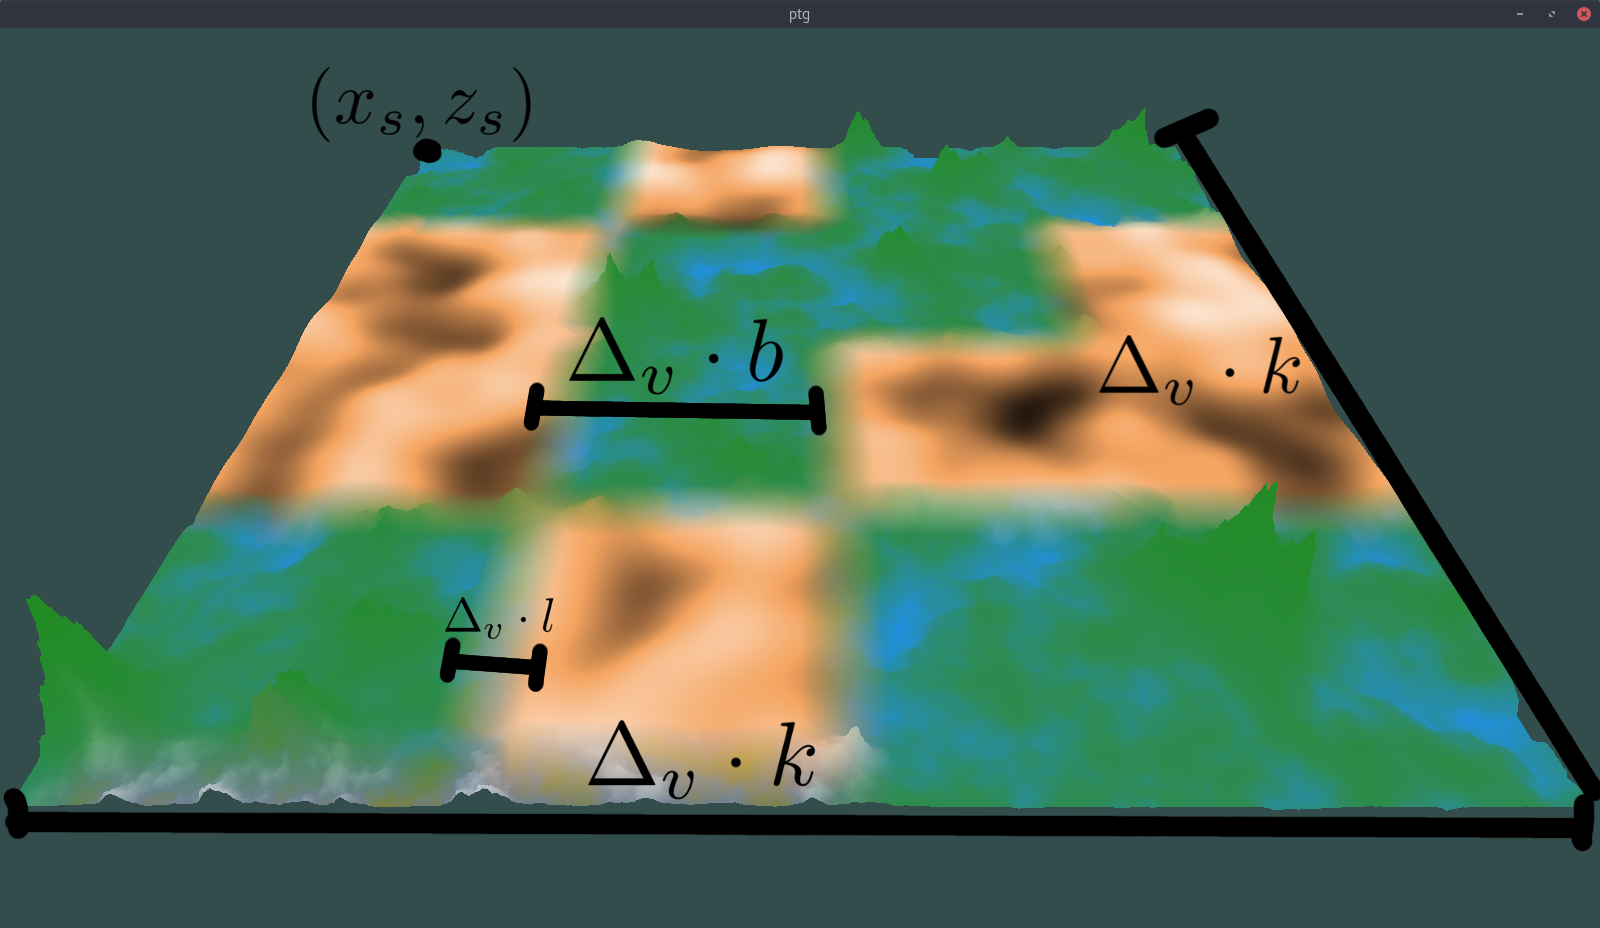
\includegraphics[width=0.75\textwidth]{figuras/resultados/sseditada.png}
%    \caption{sseditada}
%    \label{fig:sseditada}
%\end{figure}
\begin{figure}[H]
     \centering
     \subfloat[][$biomaTipo =$ Planícies]{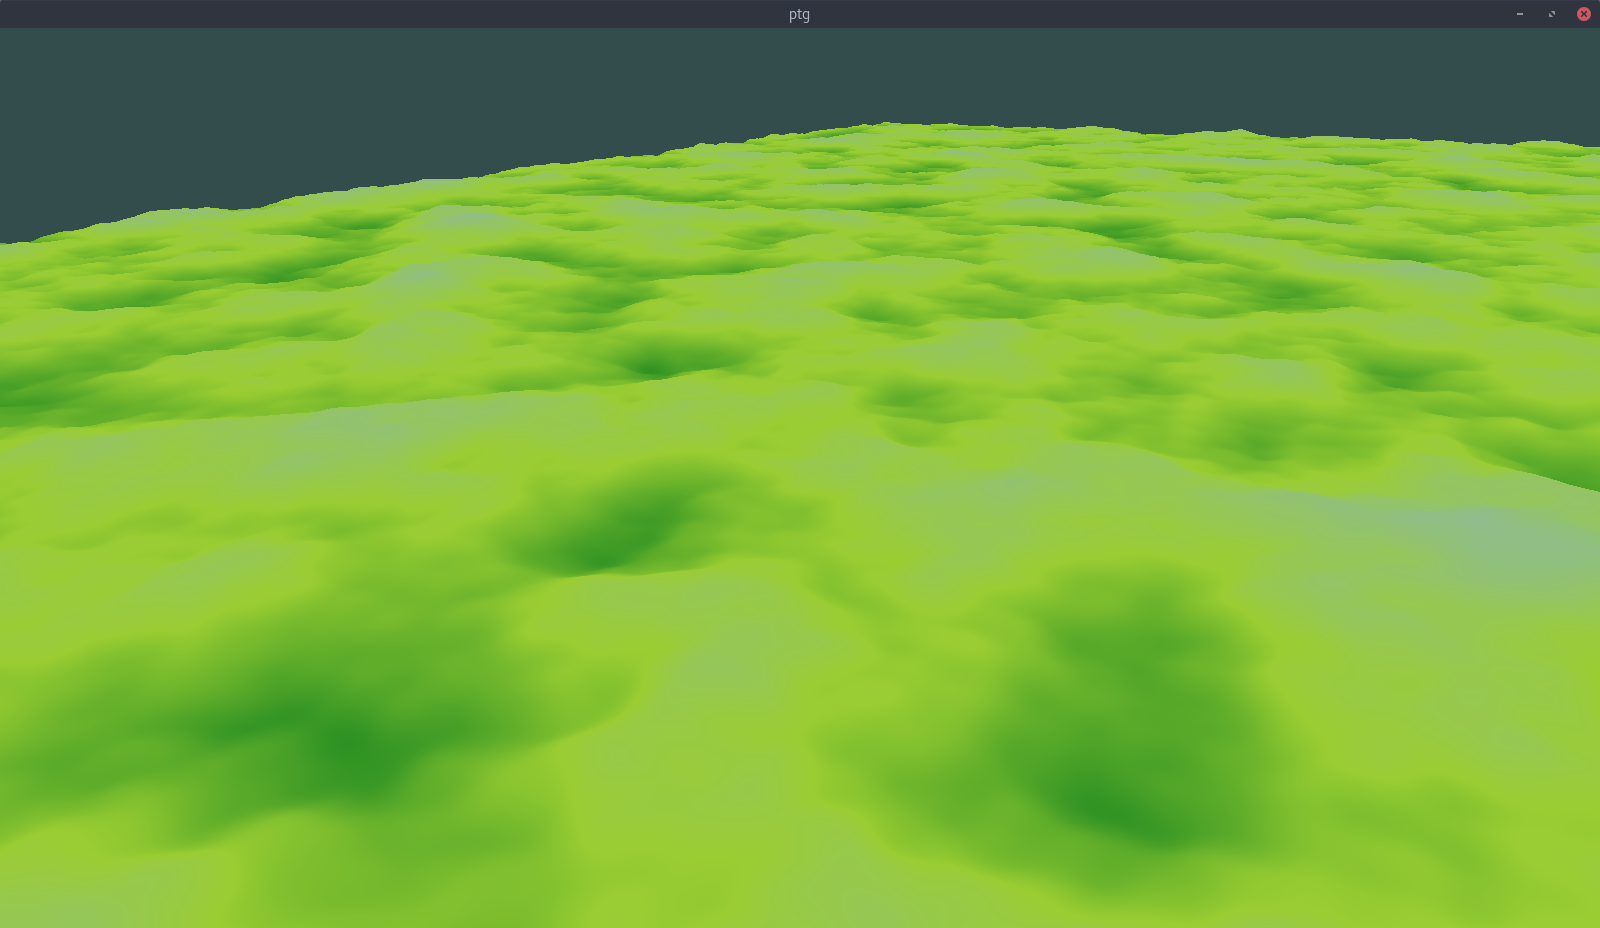
\includegraphics[width=0.48\textwidth]{figuras/bssPlains.png}\label{fig:biomaTipo1}}\hspace{0.1cm}
     \subfloat[][$biomaTipo =$ Montanhas]{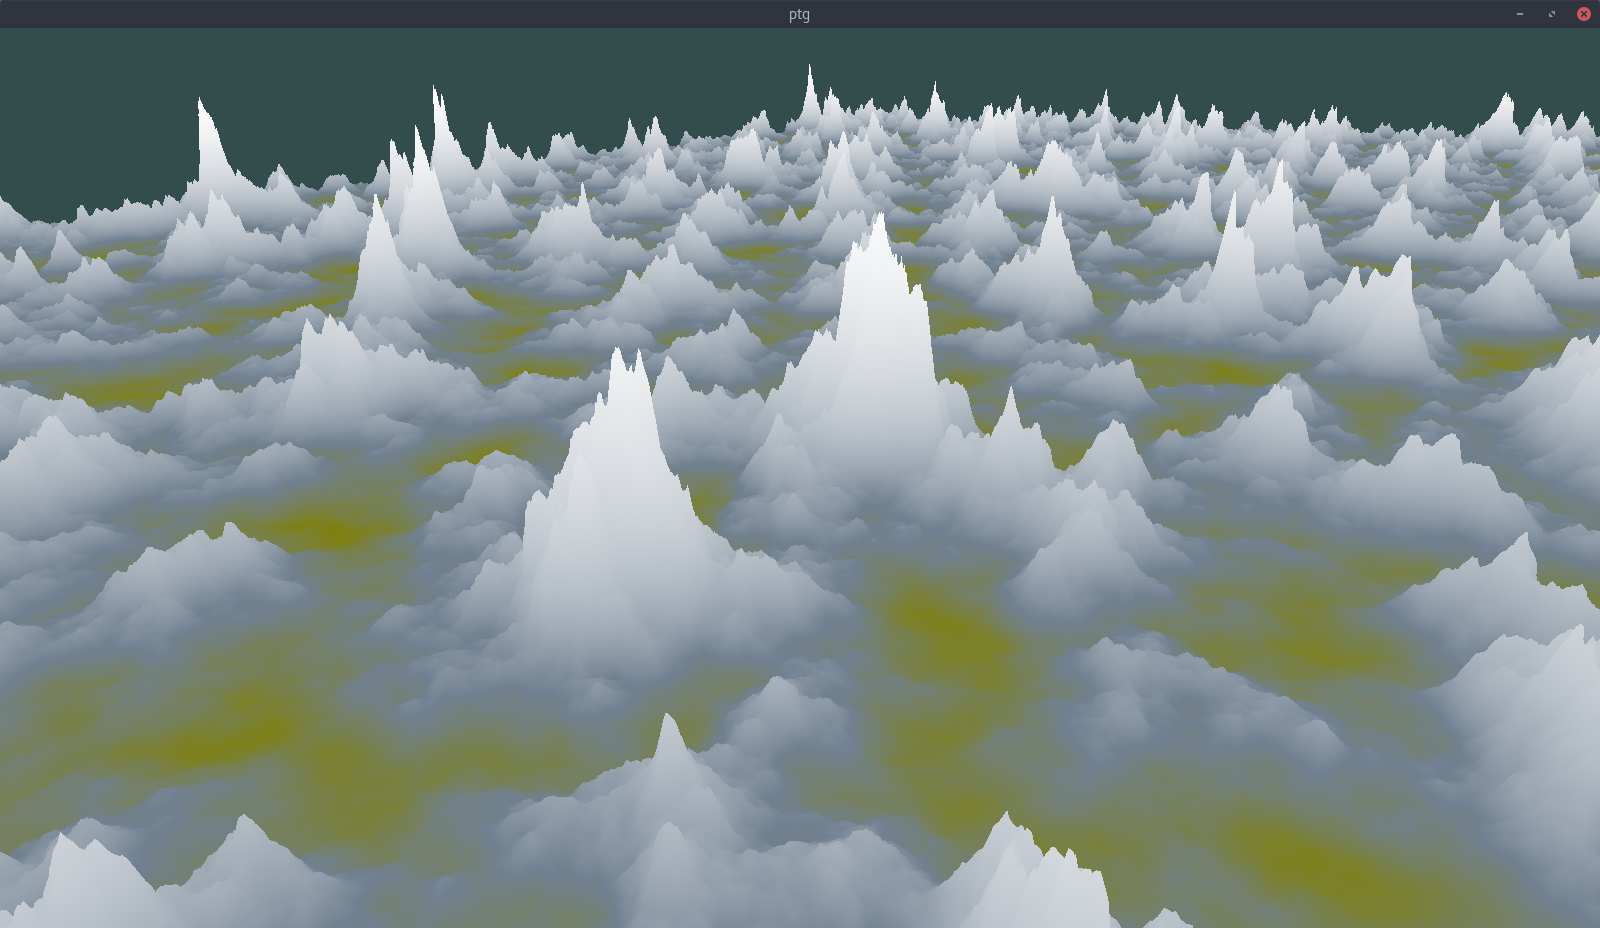
\includegraphics[width=0.48\textwidth]{figuras/bssMontains.png}\label{fig:biomaTipo2}}\\
     \subfloat[][$biomaTipo =$ Vales]{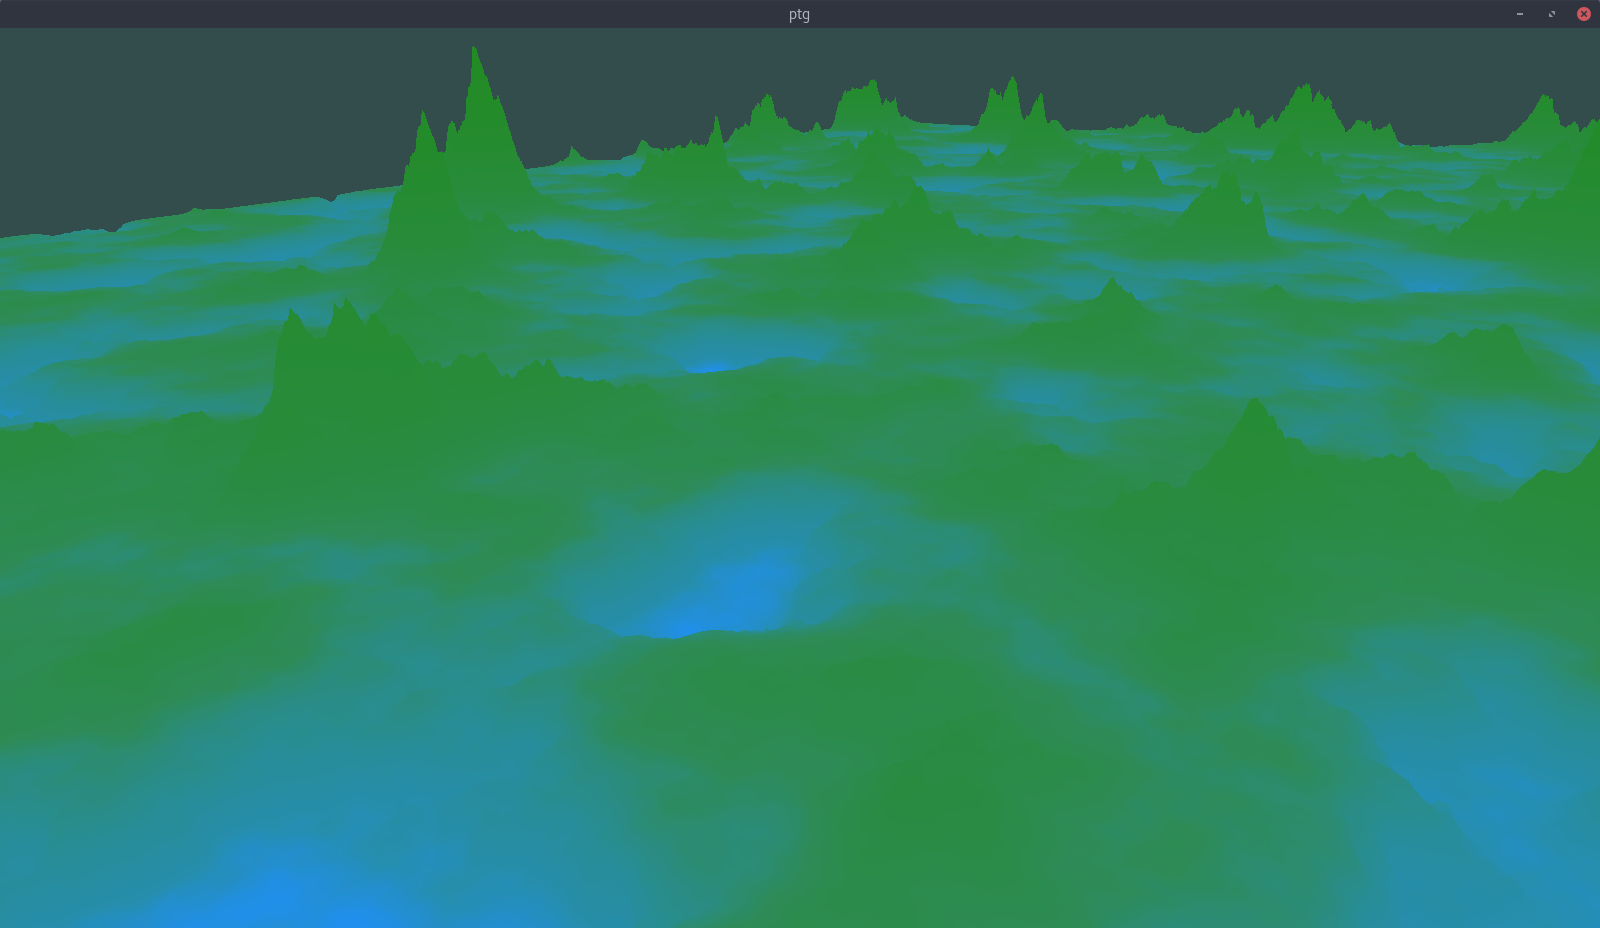
\includegraphics[width=0.48\textwidth]{figuras/bssValley.png}\label{fig:biomaTipo3}}\hspace{0.1cm}
     \subfloat[][$biomaTipo =$ Deserto]{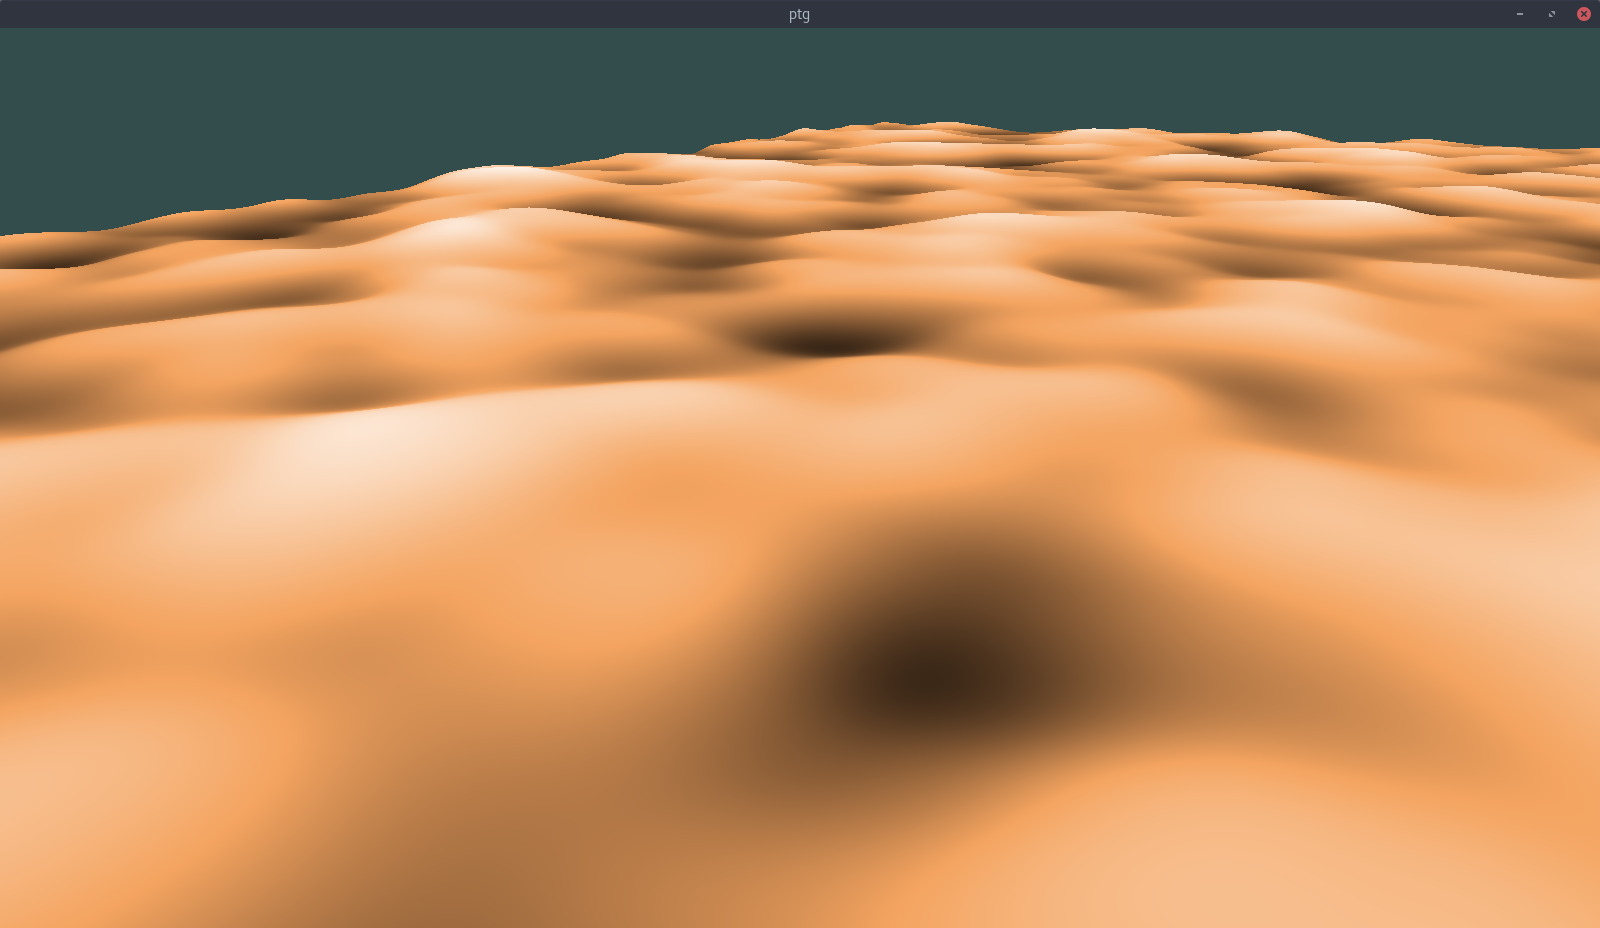
\includegraphics[width=0.48\textwidth]{figuras/bssDesert.png}\label{fig:biomaTipo4}}\\
     \subfloat[][$biomaTipo =$ Cânyons]{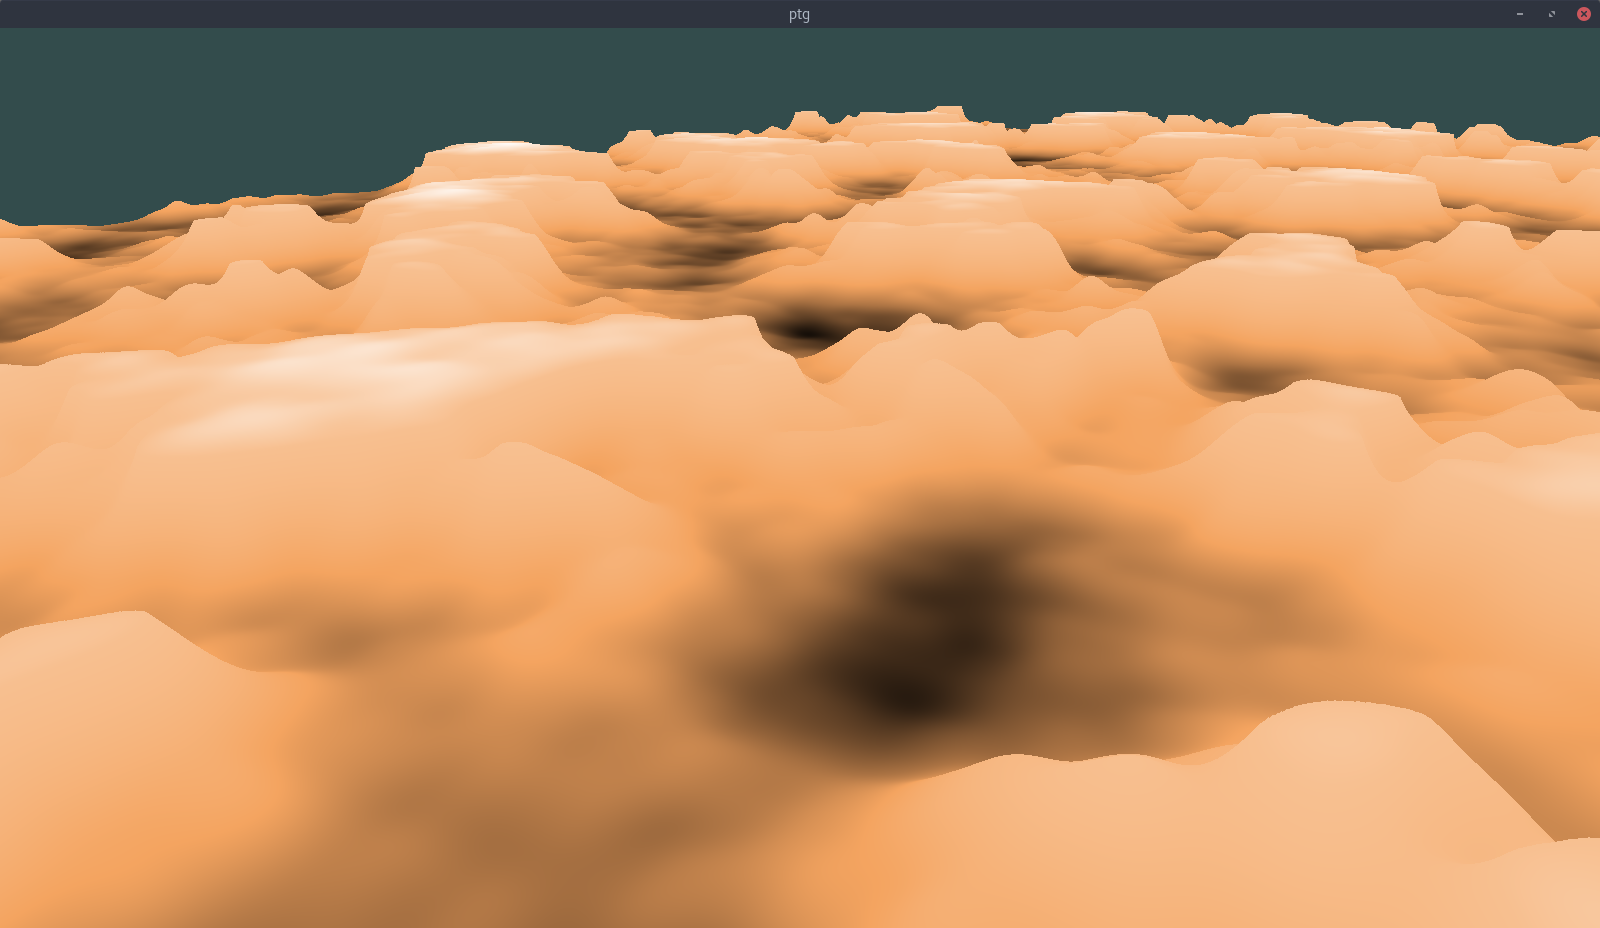
\includegraphics[width=0.48\textwidth]{figuras/bssCanyons.png}\label{fig:biomaTipo5}}
     
     \caption{Resultado dos Biomas fixados.}
     
     \label{fig:bssComBiomasFixados}
     % usar \hspace{0.1cm}, é gambiarra mas funciona
\end{figure}

As regiões dos biomas são separadas em áreas quadradas de proporção $b$, para definir
qual bioma pertence a cada área é usado o ruído, mas dessa vez a entrada se dá por valores
truncados da localização dividida por $b$ e temos o parâmetro $fb$ que define a frequência nas
mudanças de bioma. A influência destes parâmetros podem ser visualizados nas imagens \ref{fig:comparandoareadebiomasyeah} e \ref{fig:comparandofreqdebiomasyeah}.

A vantagem de usar ruído para decidir qual bioma pertence a qual 
região é que ele matem próximo biomas de valores parecidos, assim como este trabalho o de
\cite{patel2010polygonal} também se aproveitou desta característica.

\begin{figure}[H]
     \centering
     \subfloat[][$b = 16$]{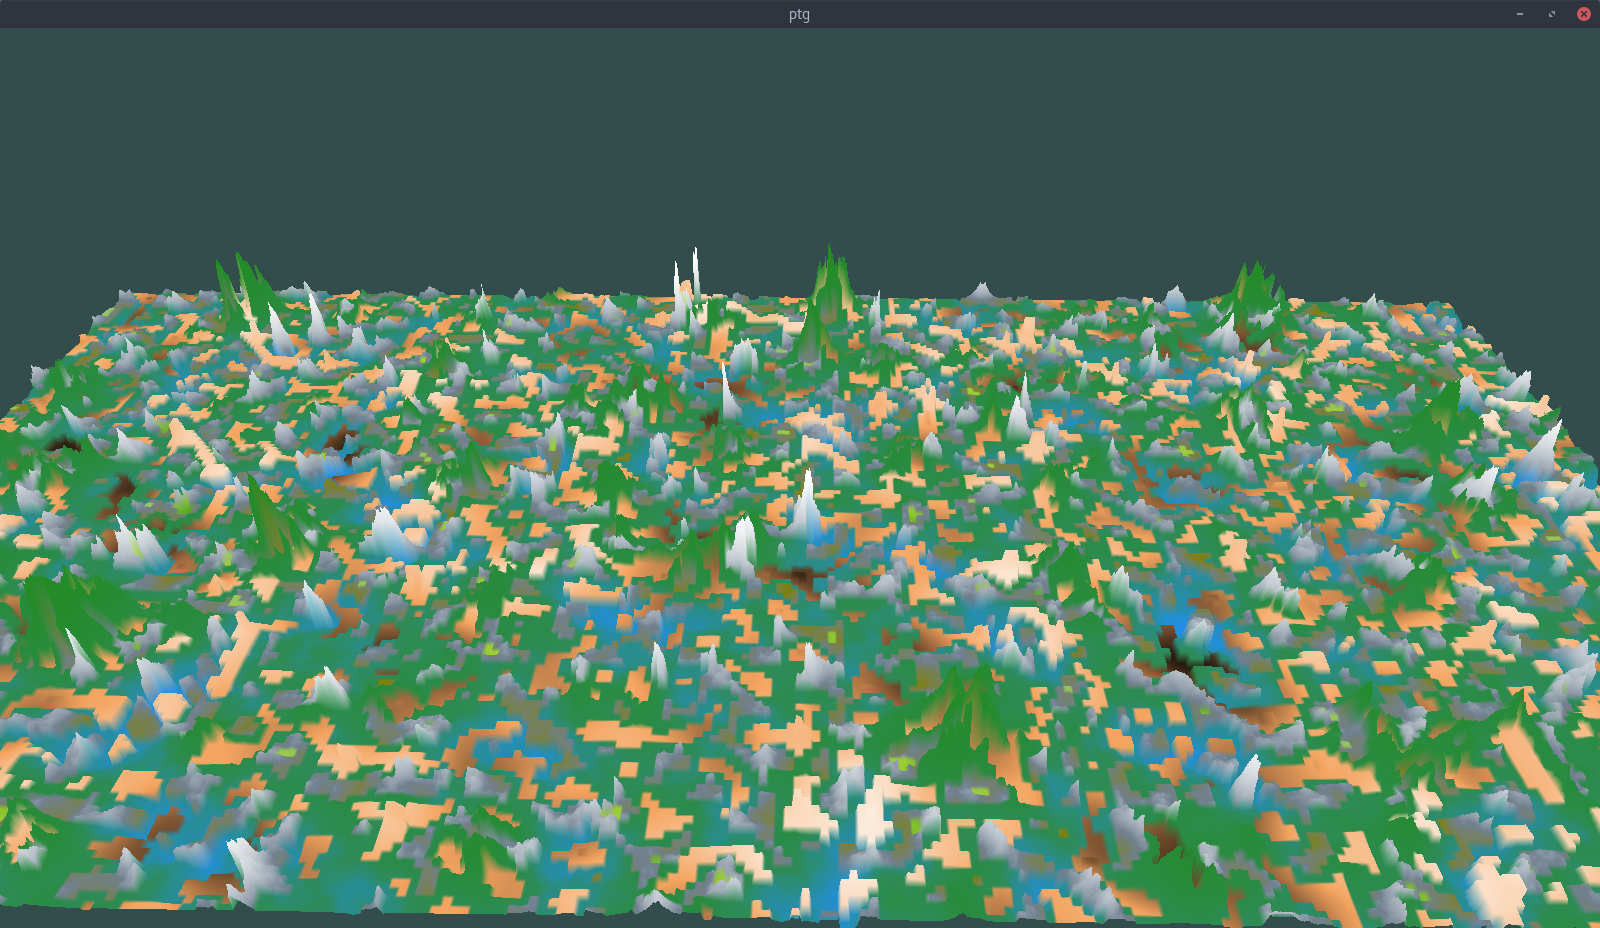
\includegraphics[width=0.31\textwidth]{figuras/re2bfb/b/16f4.png}\label{fig:re2bfb_b_16f4}}\hspace{0.1cm}
     \subfloat[][$b = 32$]{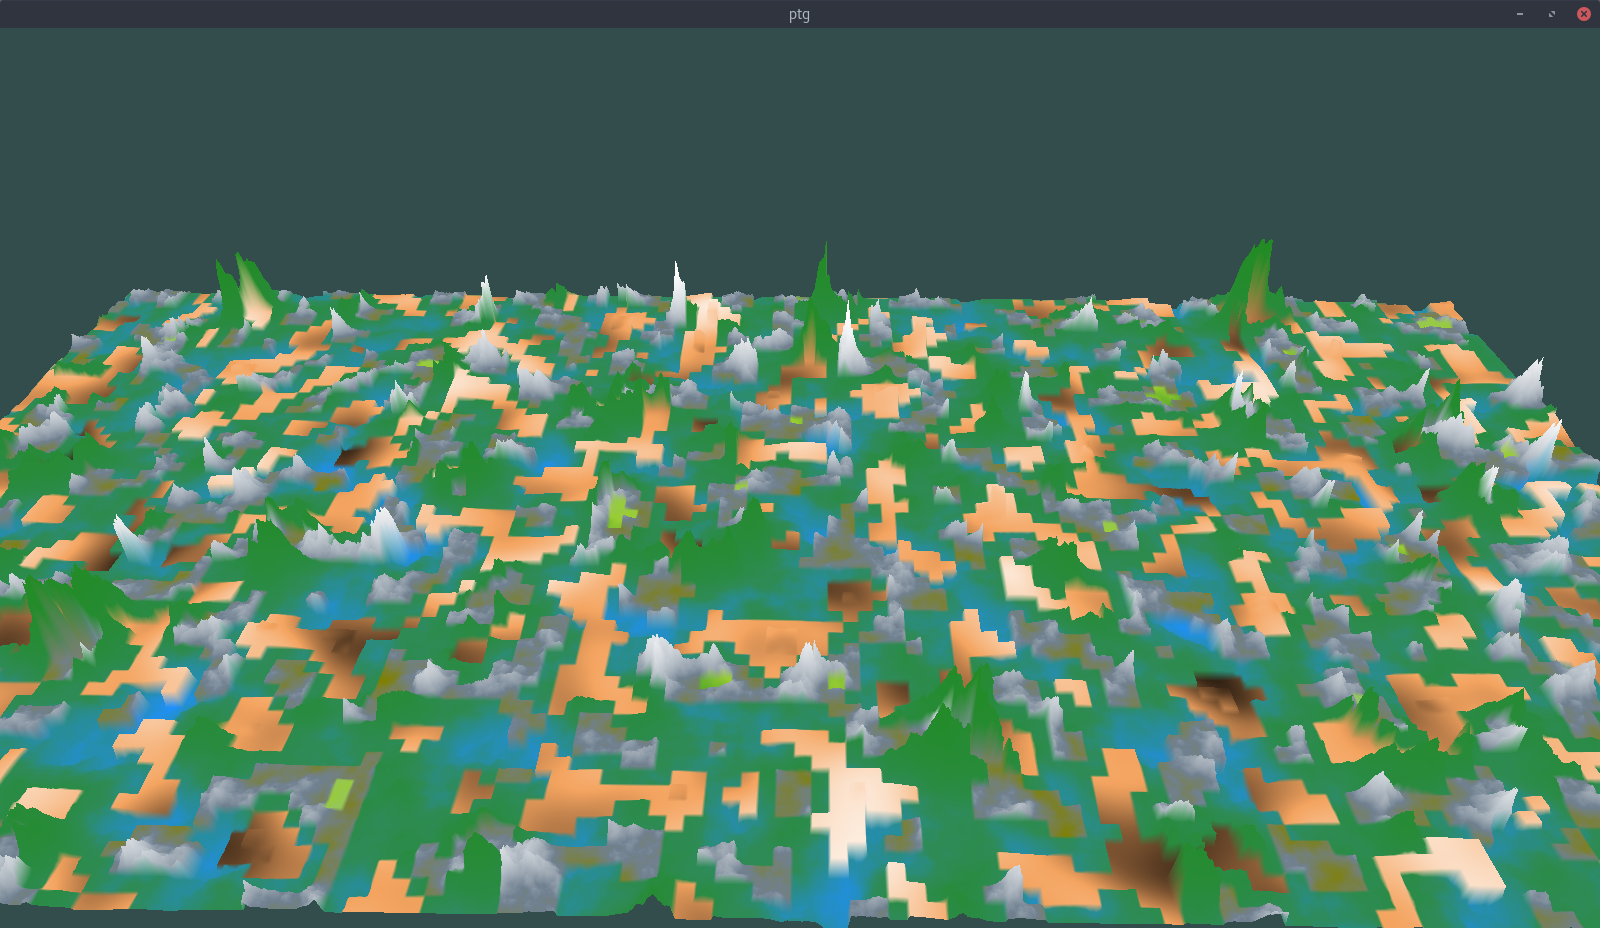
\includegraphics[width=0.31\textwidth]{figuras/re2bfb/b/32f4.png}\label{fig:re2bfb_b_32f4}}\hspace{0.1cm}
     \subfloat[][$b = 64$]{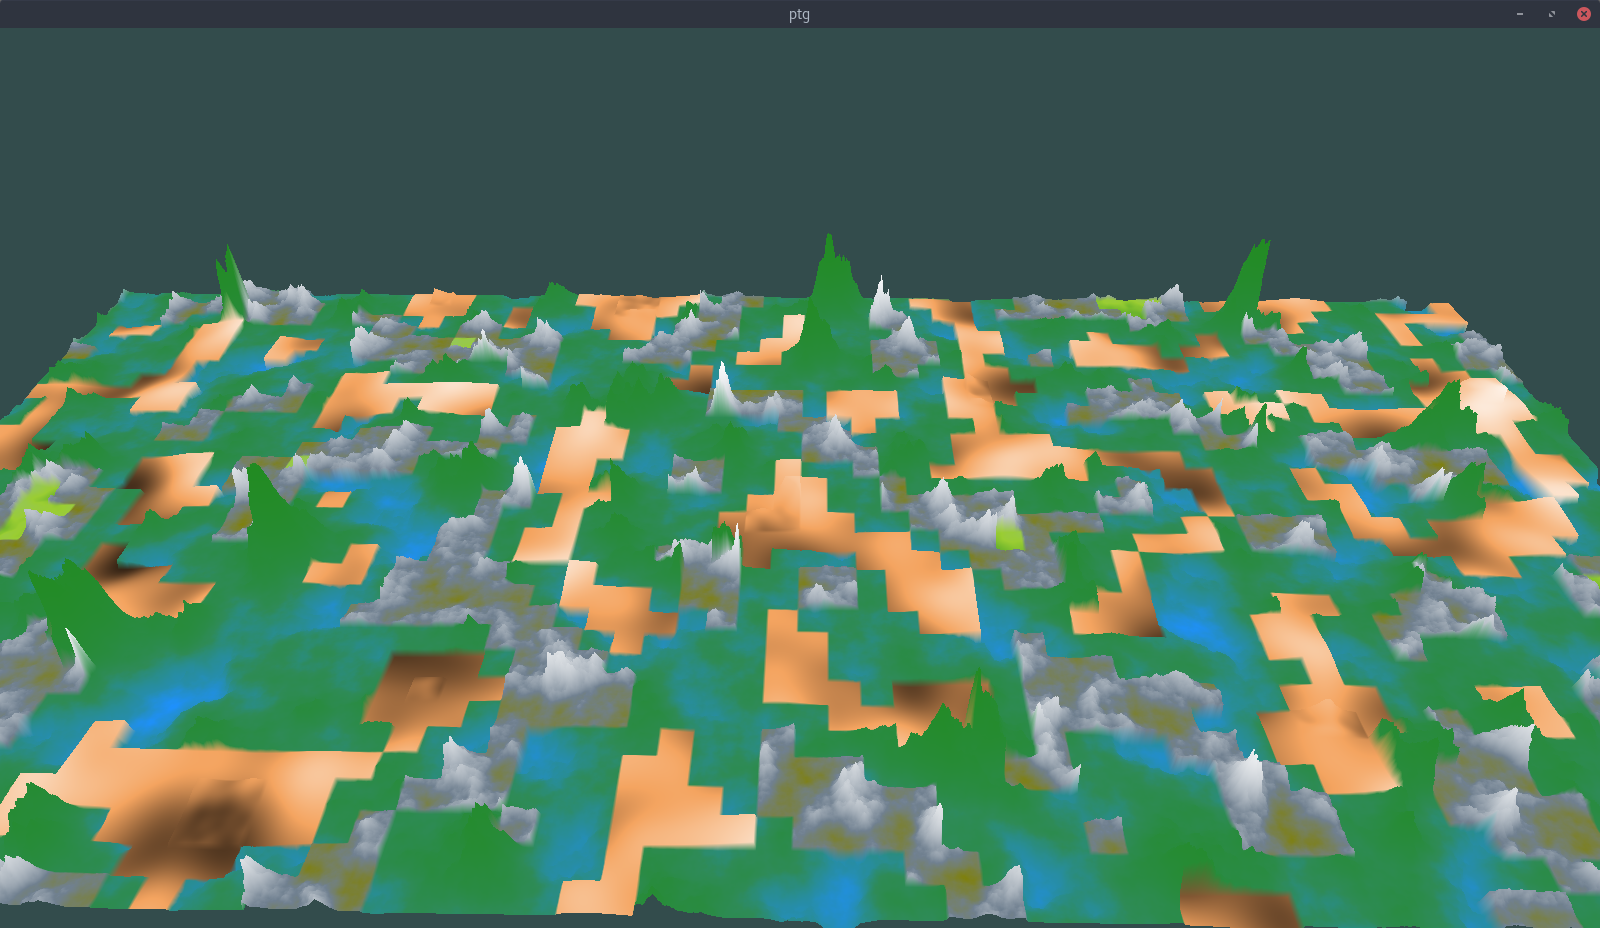
\includegraphics[width=0.31\textwidth]{figuras/re2bfb/b/64f4.png}\label{fig:re2bfb_b_64f4}}\\
     \subfloat[][$b = 128$]{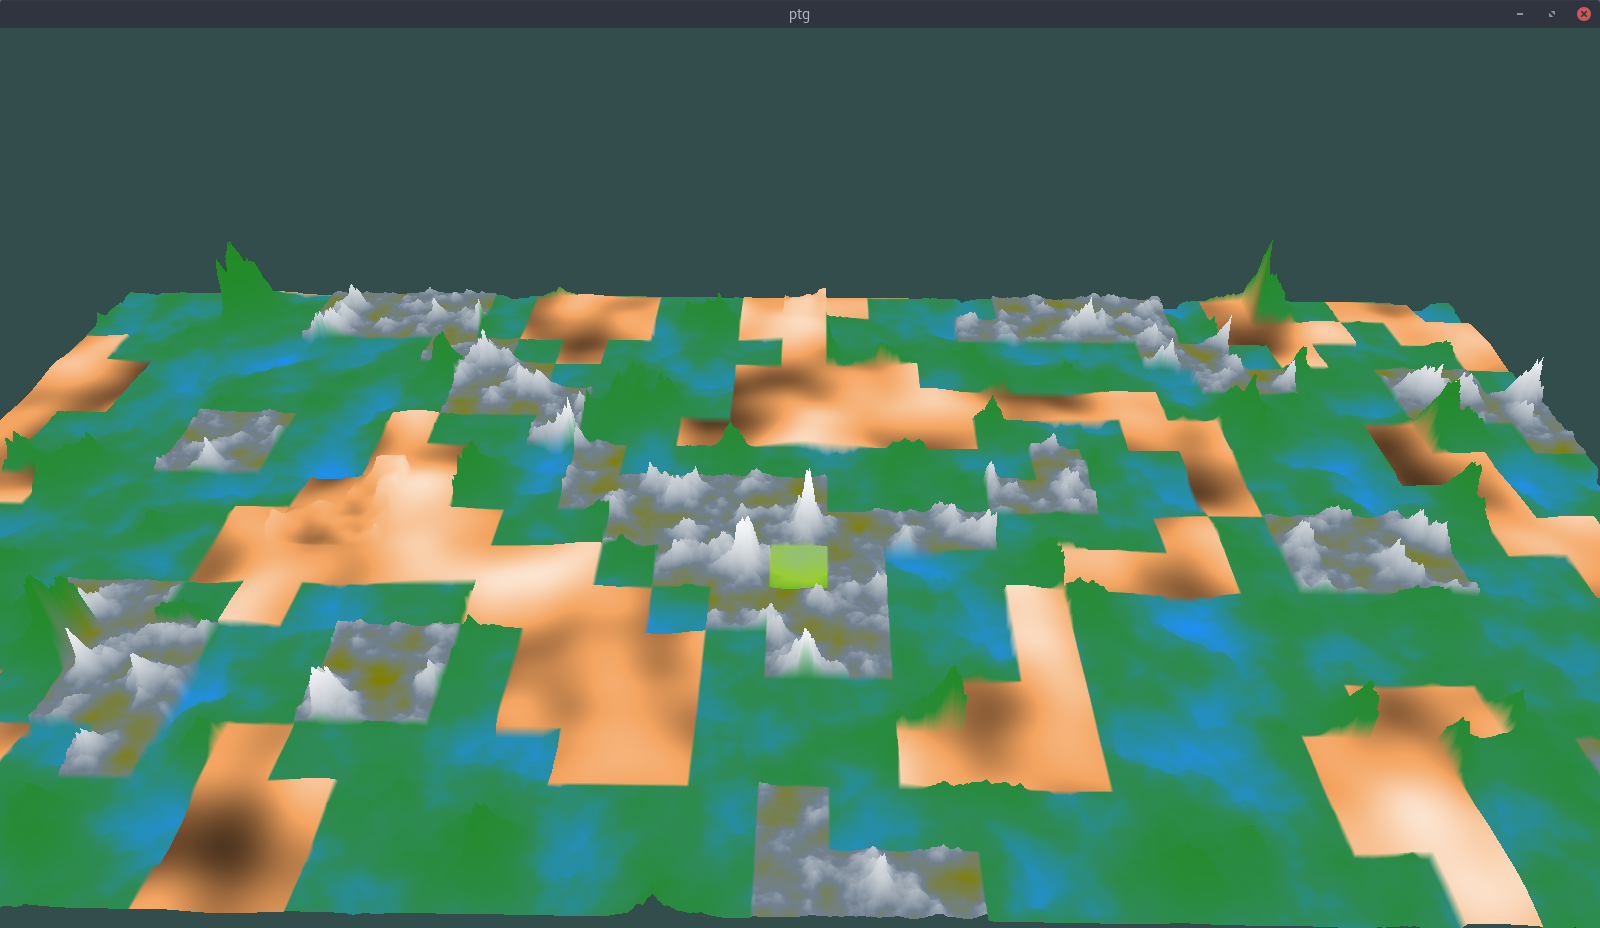
\includegraphics[width=0.31\textwidth]{figuras/re2bfb/b/128f4.png}\label{fig:re2bfb_b_128f4}}\hspace{0.1cm}
     \subfloat[][$b = 256$]{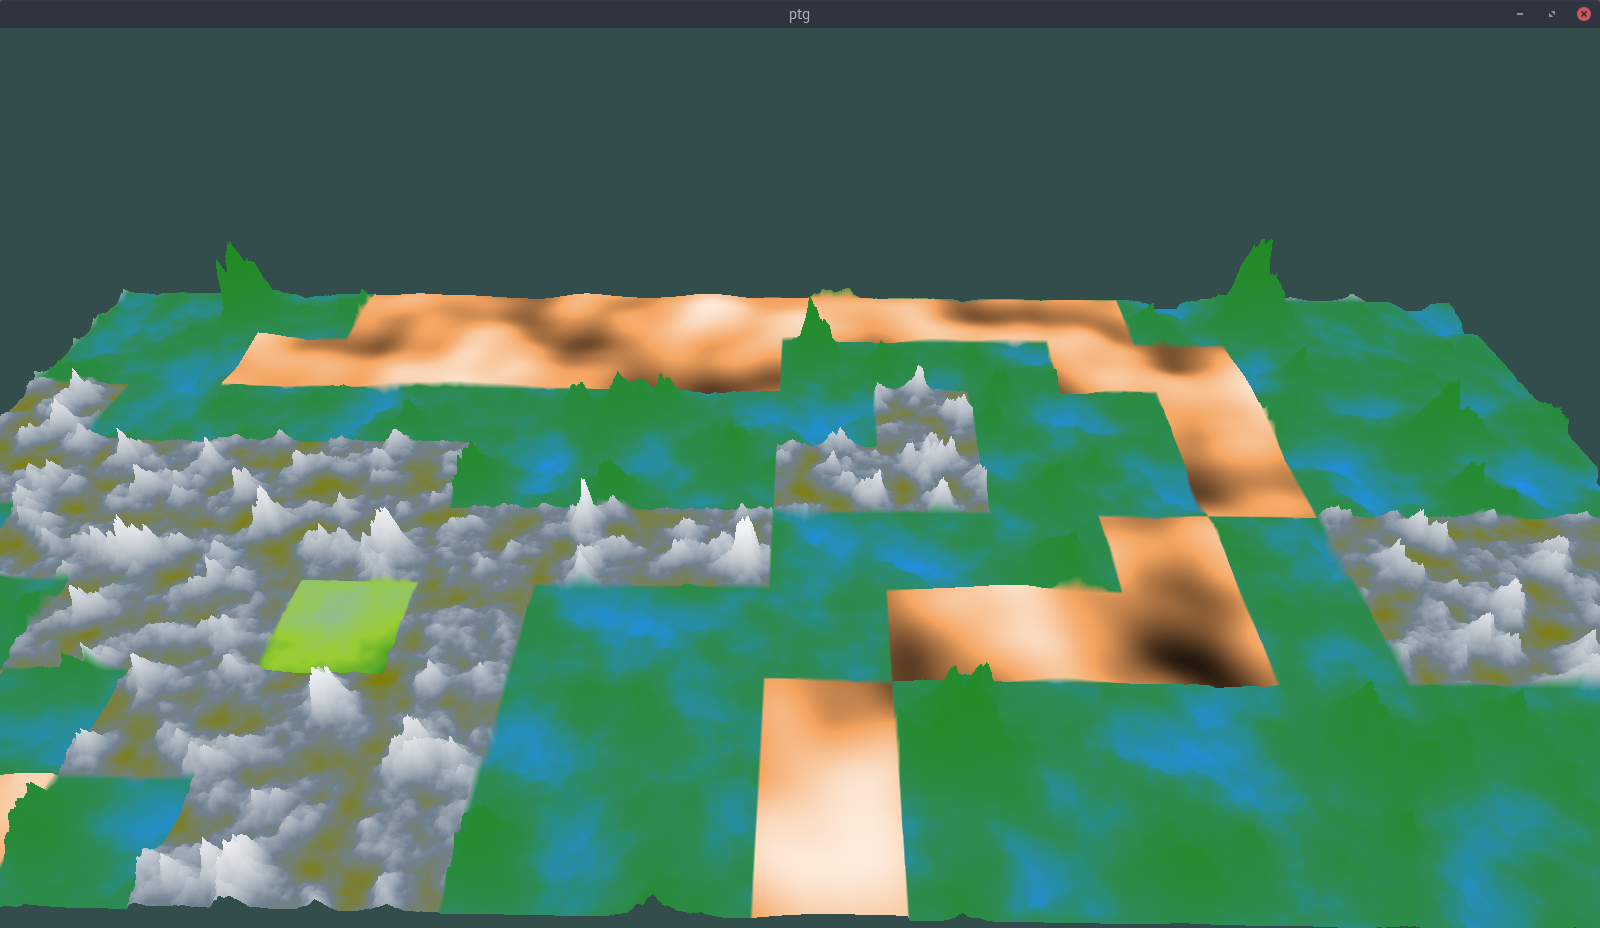
\includegraphics[width=0.31\textwidth]{figuras/re2bfb/b/256f4.png}\label{fig:re2bfb_b_256f4}}\hspace{0.1cm}
     \subfloat[][$b = 512$]{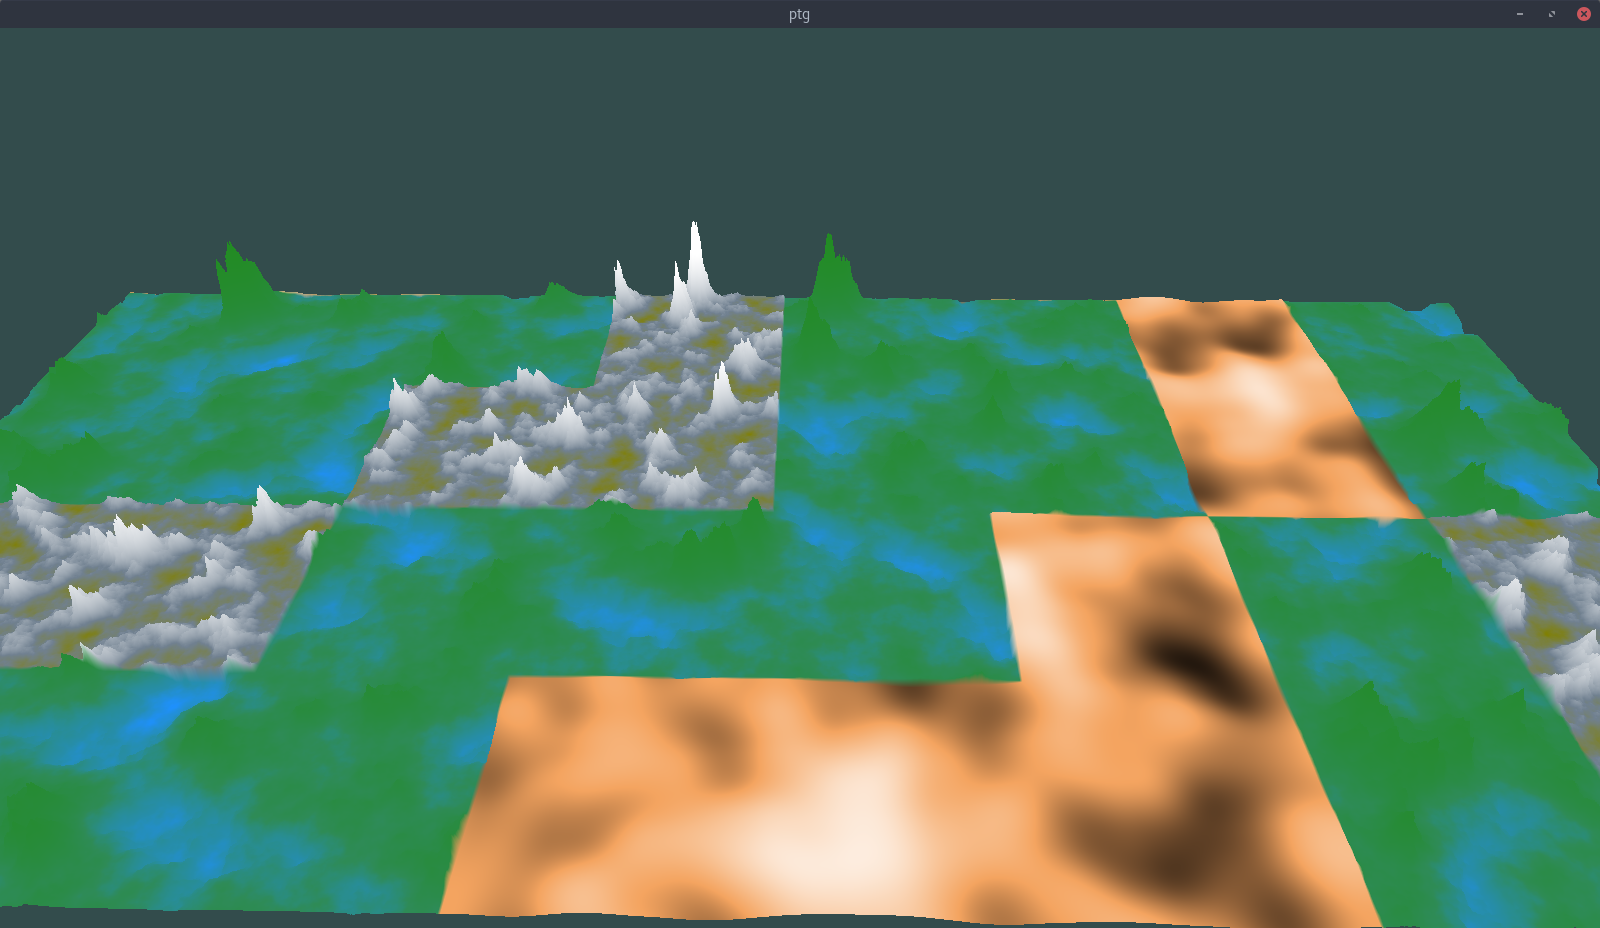
\includegraphics[width=0.31\textwidth]{figuras/re2bfb/b/512f4.png}\label{fig:re2bfb_b_512f4}}
     
     \caption{Diferentes tamanhos para áreas de bioma($b$), usando $fb = 4$.}
     
     \label{fig:comparandoareadebiomasyeah}
     % usar \hspace{0.1cm}, é gambiarra mas funciona
\end{figure}

\begin{figure}[H]
     \centering
     \subfloat[][$fb = 0.5$]{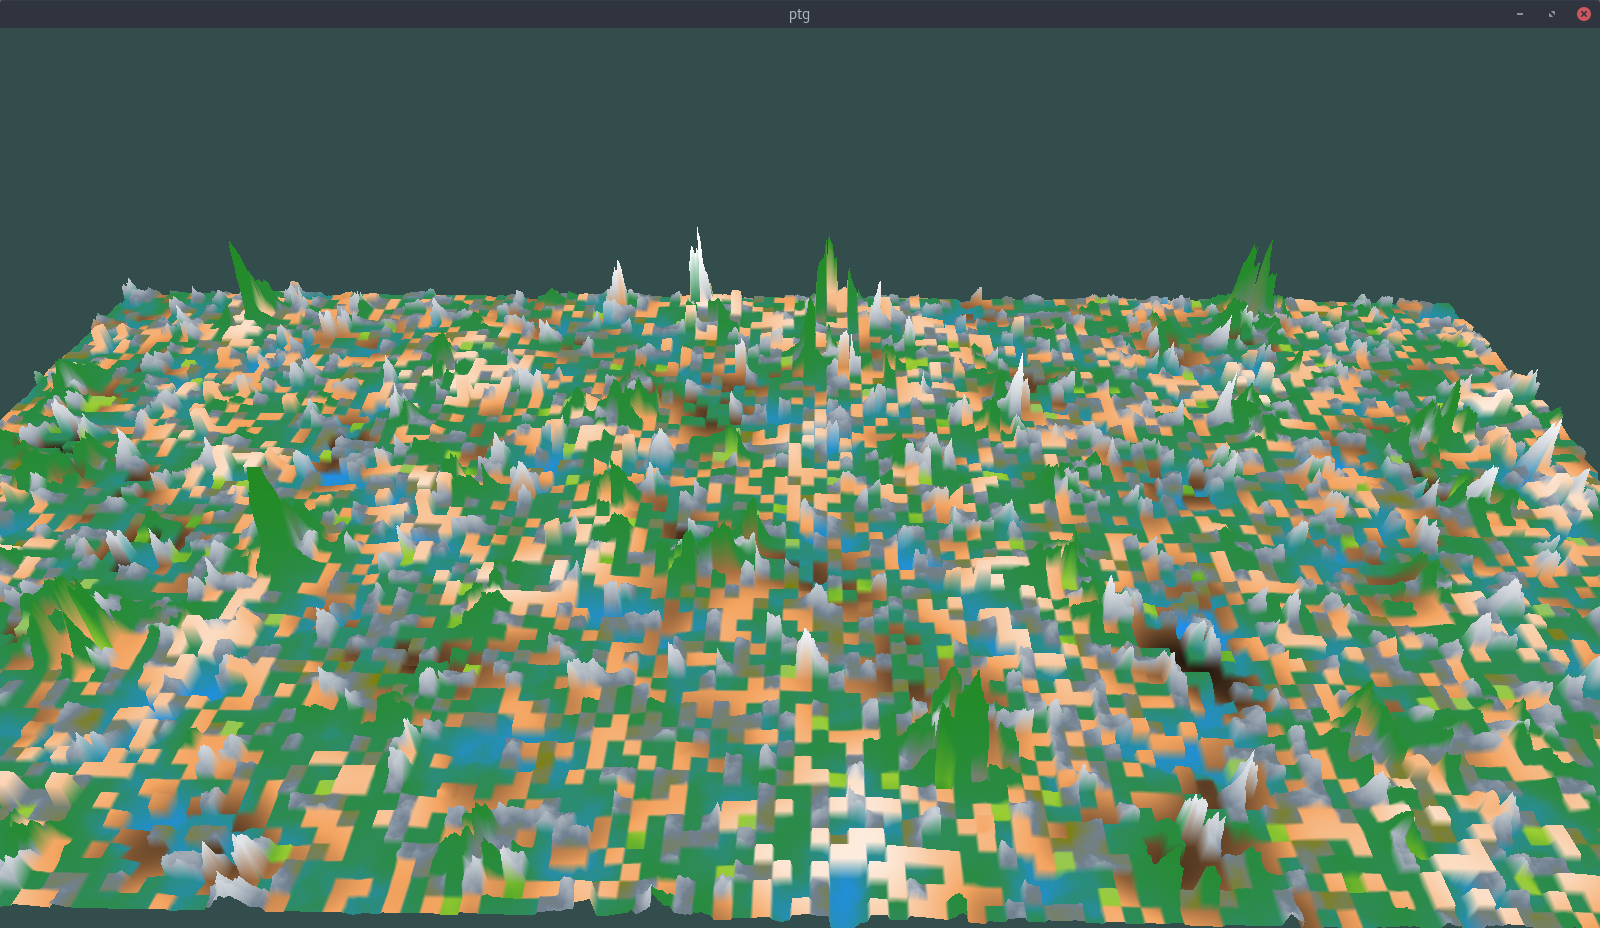
\includegraphics[width=0.31\textwidth]{figuras/re2bfb/fb/05b32.png}\label{fig:re2bfb_fb_05b32}}\hspace{0.1cm}
     \subfloat[][$fb = 1$]{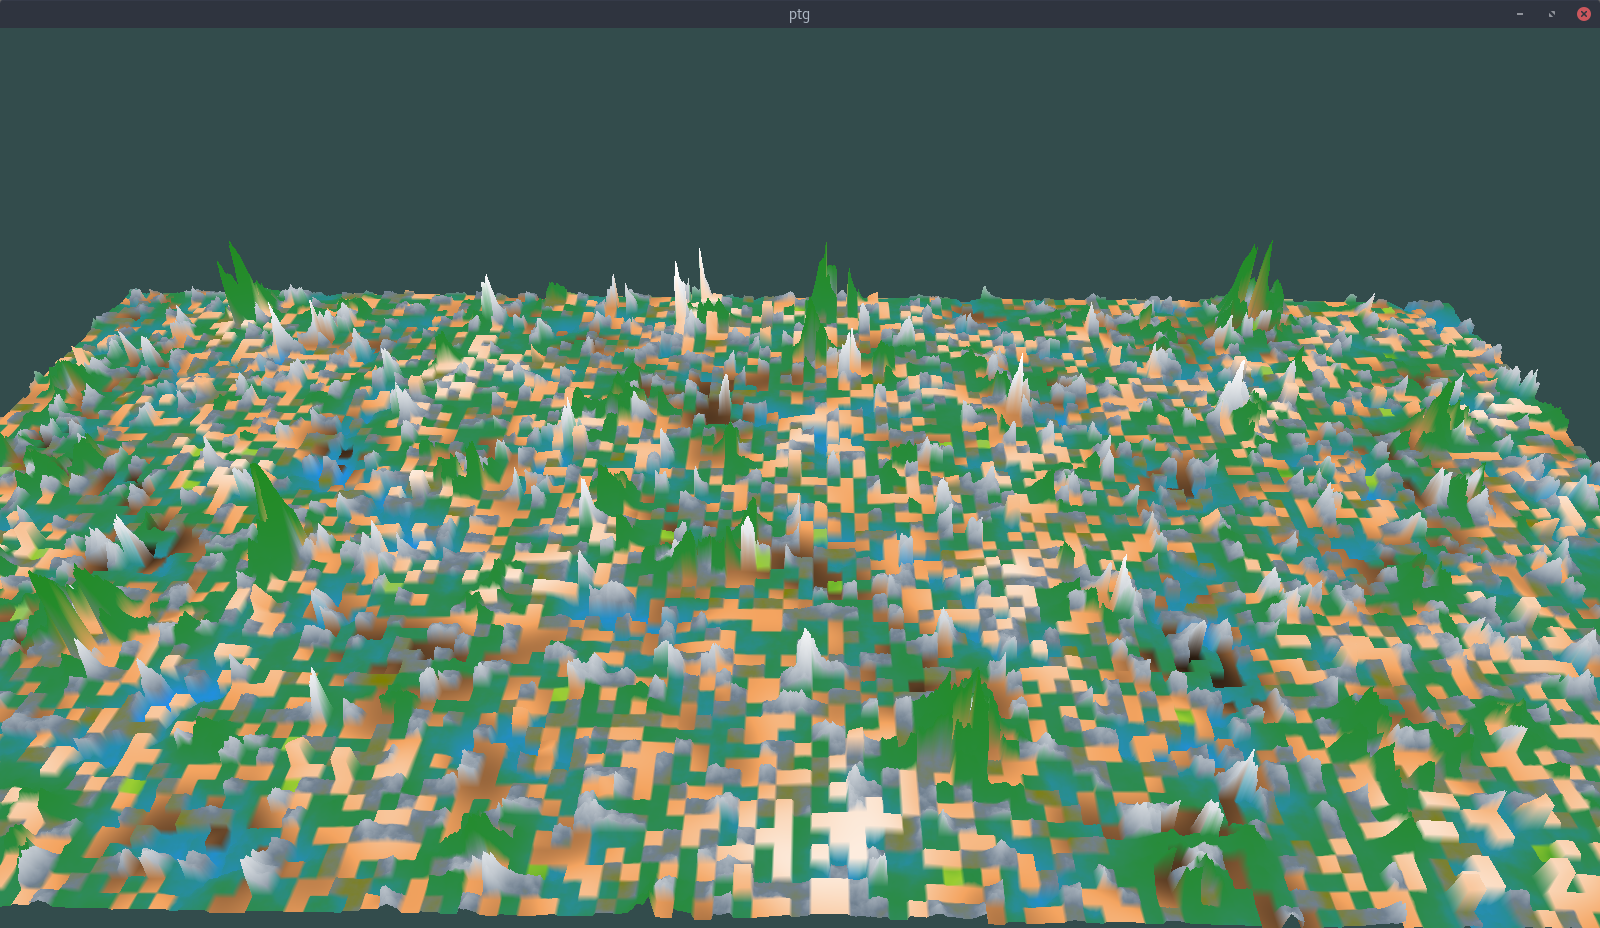
\includegraphics[width=0.31\textwidth]{figuras/re2bfb/fb/1b32.png}\label{fig:re2bfb_fb_1b32}}\hspace{0.1cm}
     \subfloat[][$fb = 8$]{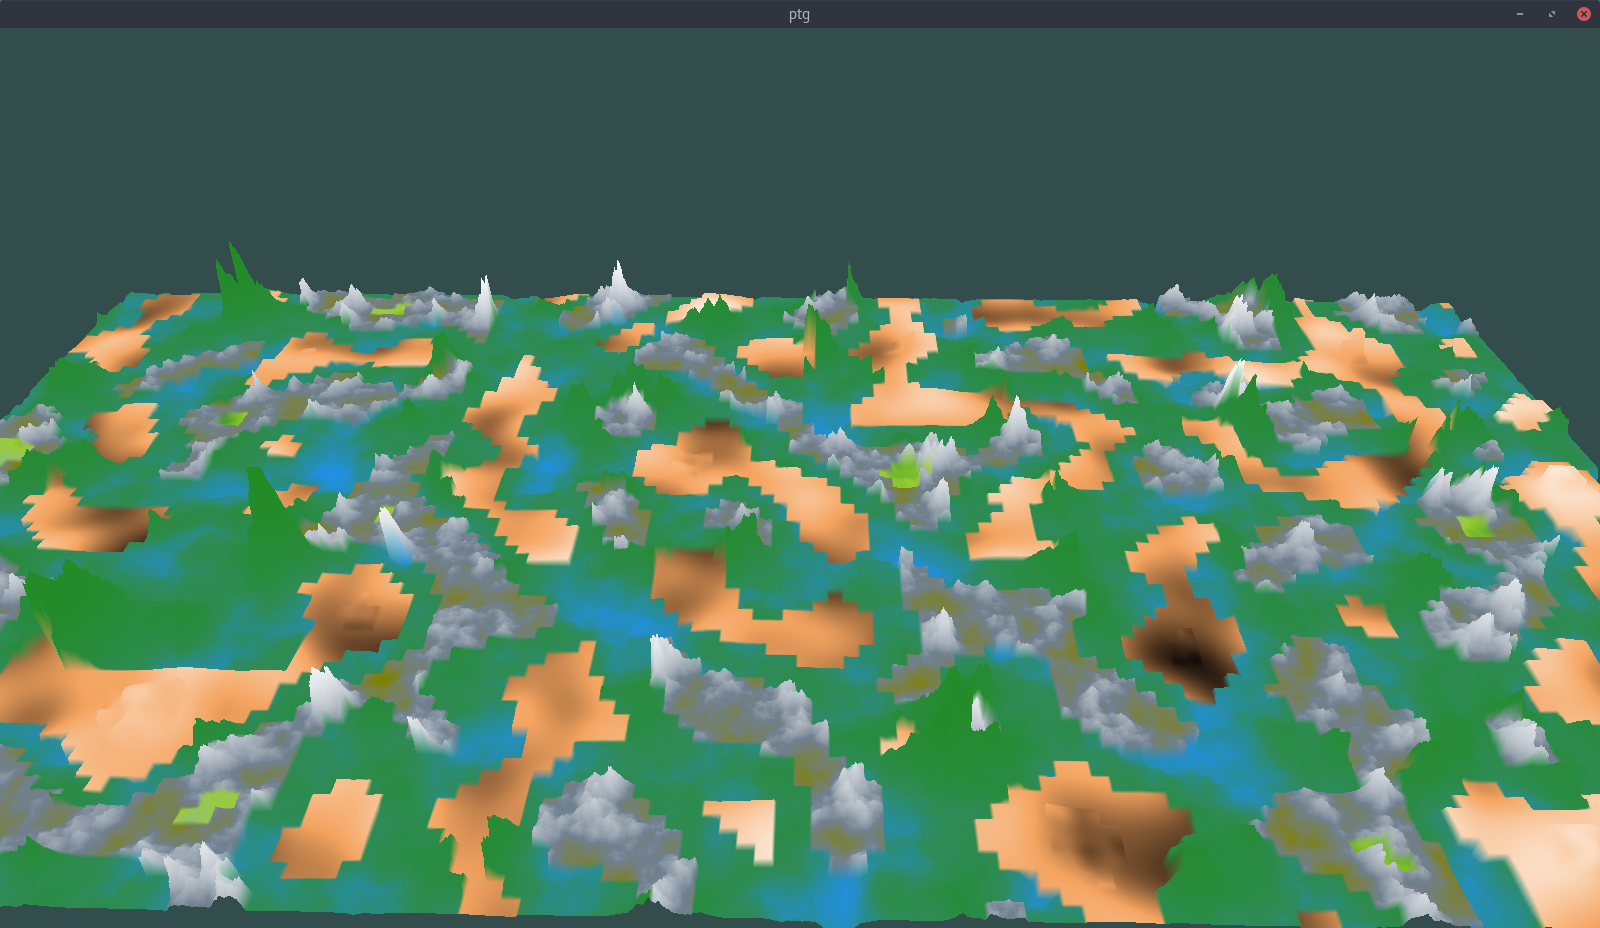
\includegraphics[width=0.31\textwidth]{figuras/re2bfb/fb/8b32.png}\label{fig:re2bfb_fb_8b32}}\\
     \subfloat[][$fb = 16$]{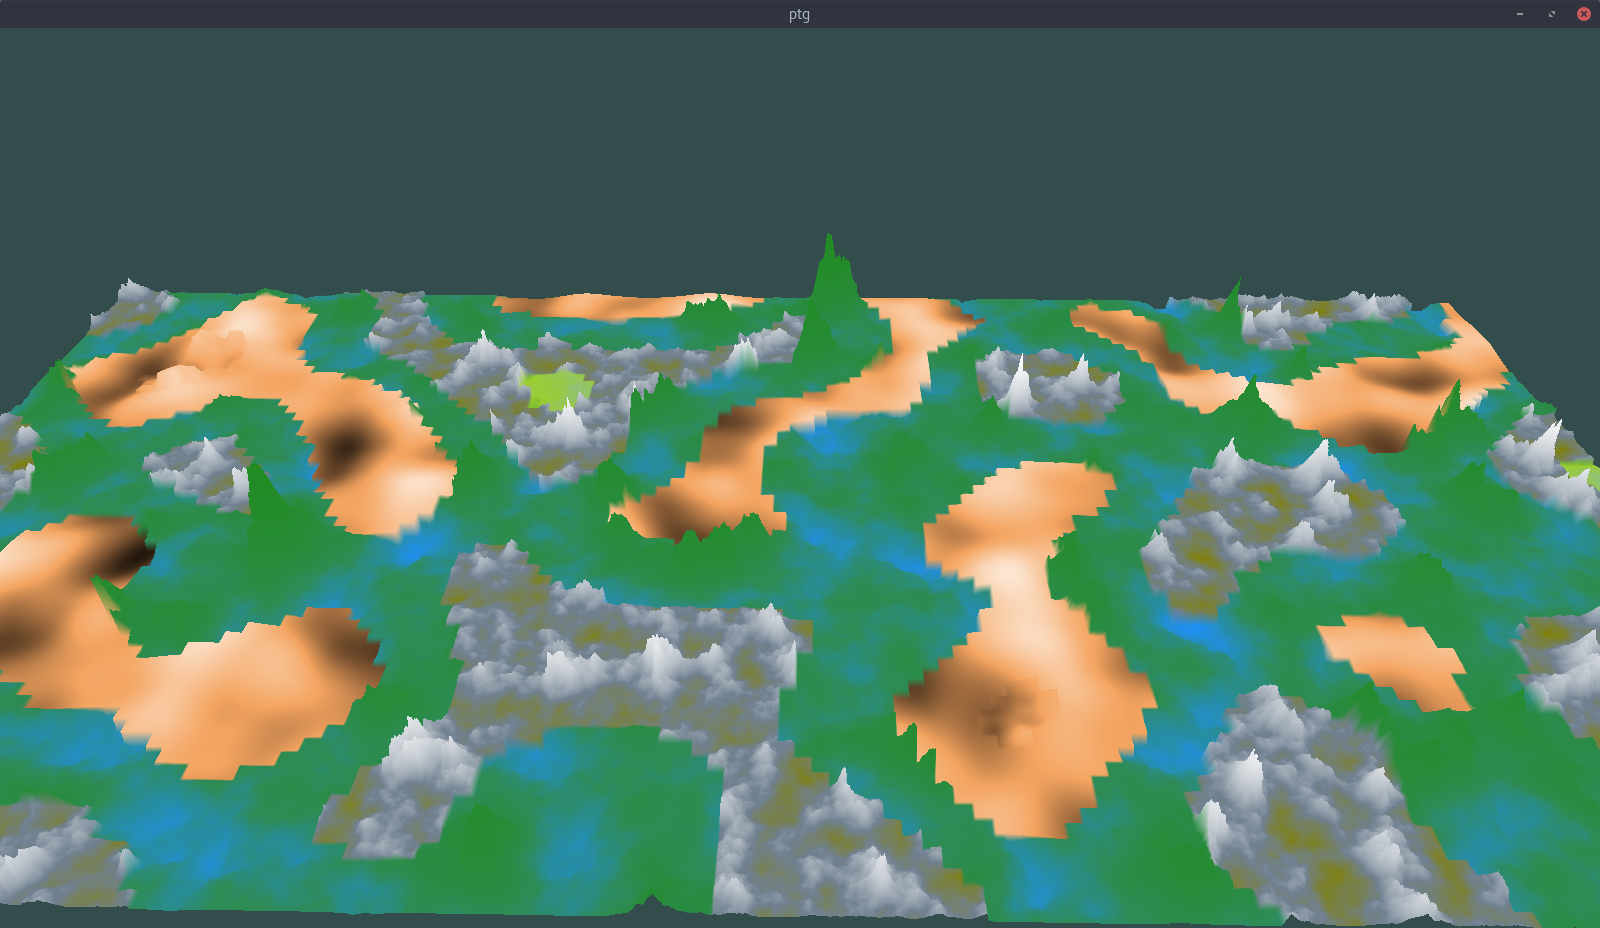
\includegraphics[width=0.31\textwidth]{figuras/re2bfb/fb/16b32.png}\label{fig:re2bfb_fb_16b32}}\hspace{0.1cm}
     \subfloat[][$fb = 32$]{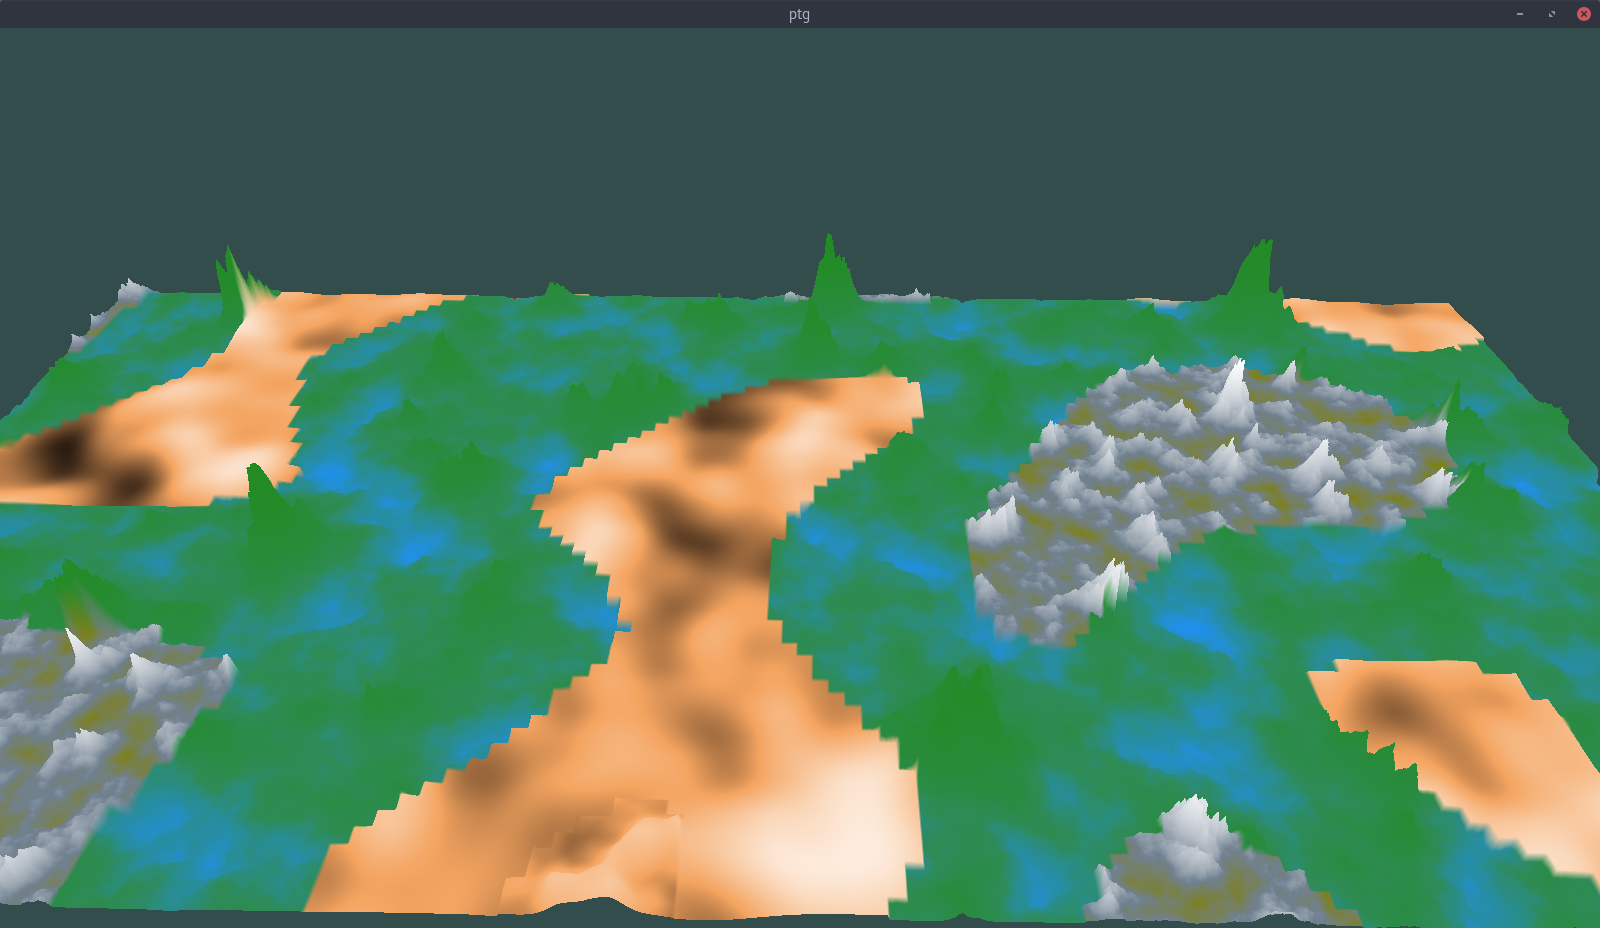
\includegraphics[width=0.31\textwidth]{figuras/re2bfb/fb/32b32.png}\label{fig:re2bfb_fb_32b32}}\hspace{0.1cm}
     \subfloat[][$fb = 64$]{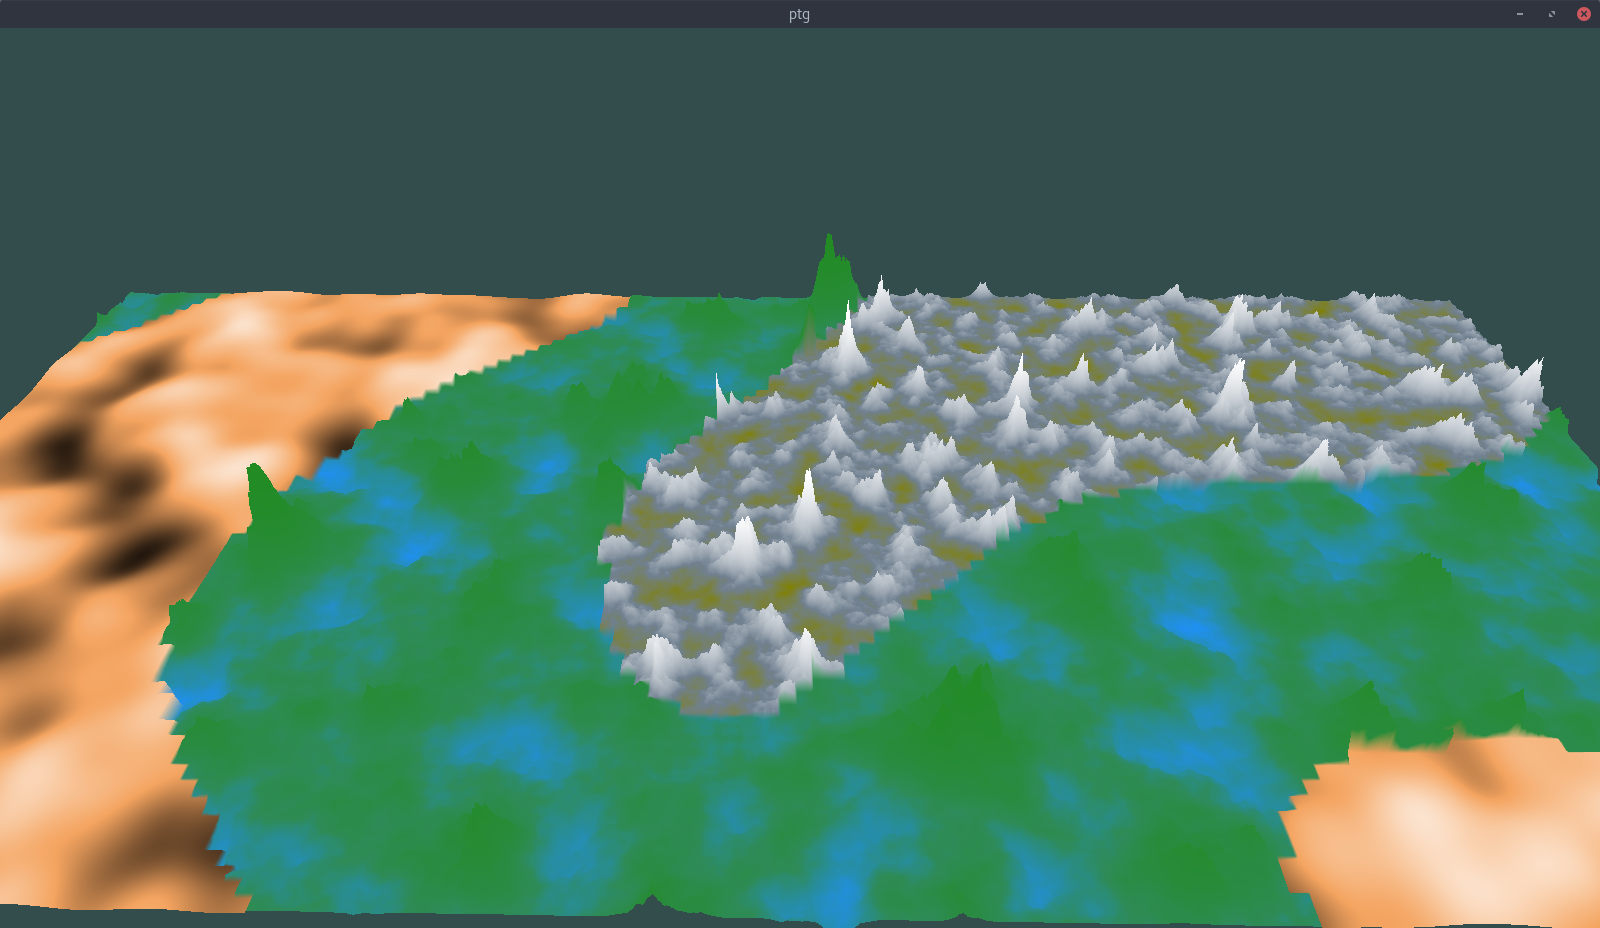
\includegraphics[width=0.31\textwidth]{figuras/re2bfb/fb/64b32.png}\label{fig:re2bfb_fb_64b32}}
     
     \caption{Diferentes frequências de biomas, para tamanho de área $b = 32$.}
     
     \label{fig:comparandofreqdebiomasyeah}
     % usar \hspace{0.1cm}, é gambiarra mas funciona
\end{figure}

Para a fronteira entre os biomas distintos obter uma forma mais orgânica, e deixar o 
terreno com melhor jogabilidade, já que descontinuidade no terreno seria um empecilho em alguns jogos.
Foi feito interpolação linear nas ocorrências de fronteiras, nas diagonais de área de bioma foi 
usado interpolação bilinear, já que este cobre o pior caso, que seria fronteira entre quatro biomas distintos,
mostrado nas figuras \ref{fig:wcborder4biomes}.%debug: figura pior caso ref aqui

A distância em que uma interpolação começa a ser feita é definida pelo parâmetro $l$,
quanto maior for $l$ maior será a área de interpolação e mais suave será transição de um bioma para o outro,
sua influência pode ser comparada nas imagens \ref{fig:borderslcomp}.

\begin{figure}[H]
     \centering
     \subfloat[][Sem interpolação]{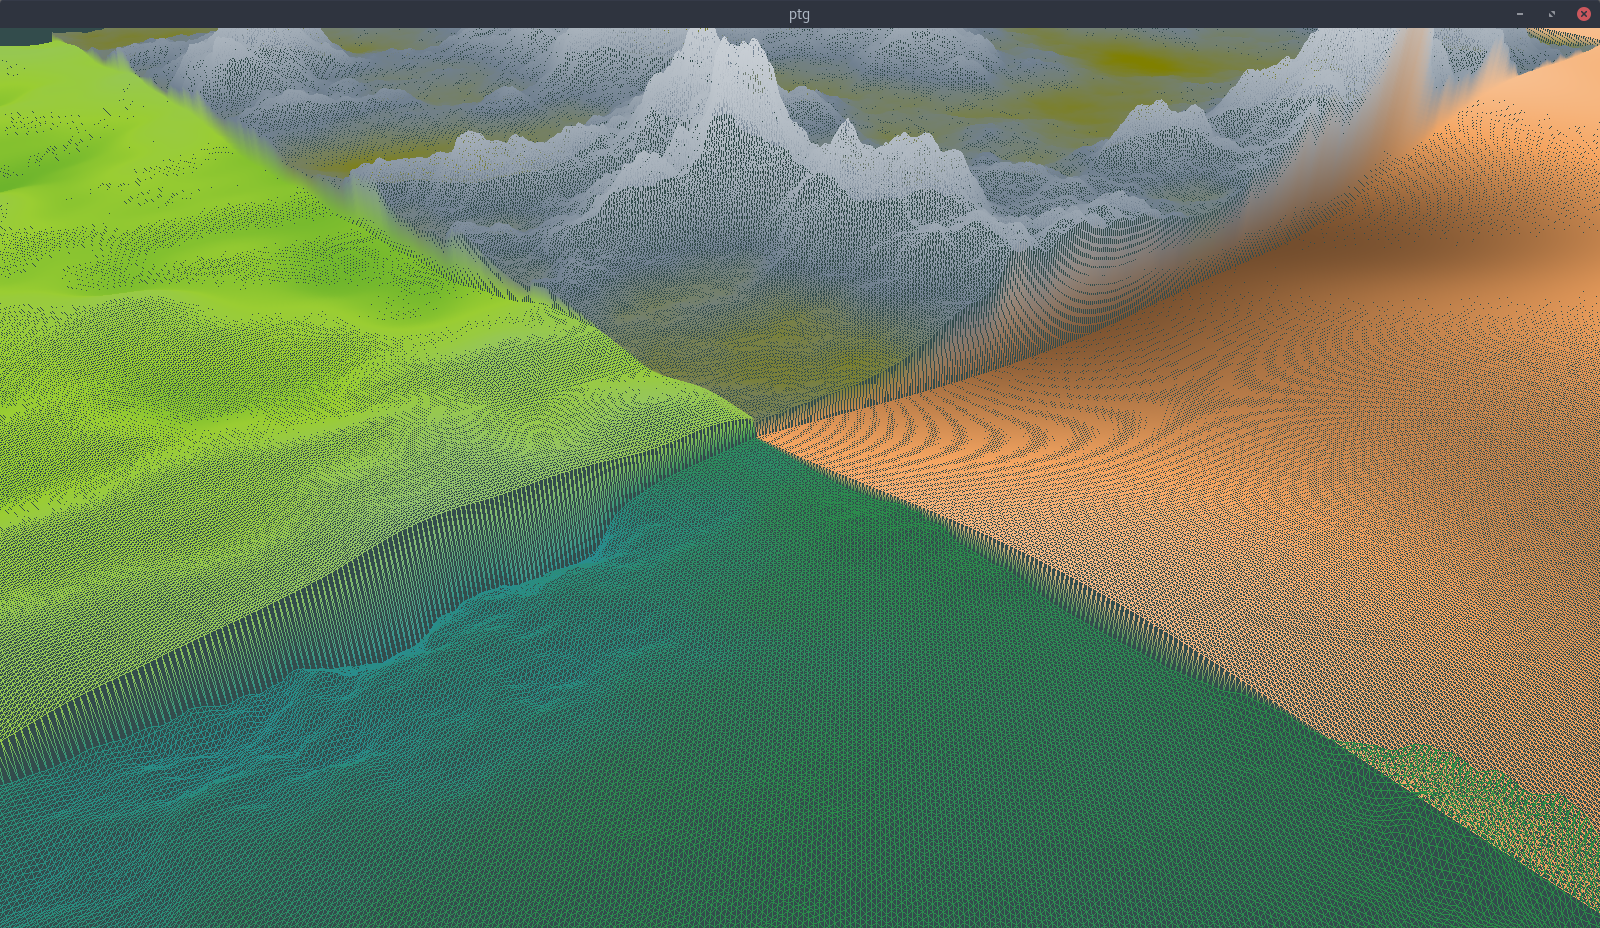
\includegraphics[width=0.48\textwidth]{figuras/wc/wcmni.png}\label{fig:wc_wcmni}}\hspace{0.1cm}
     \subfloat[][Com interpolação]{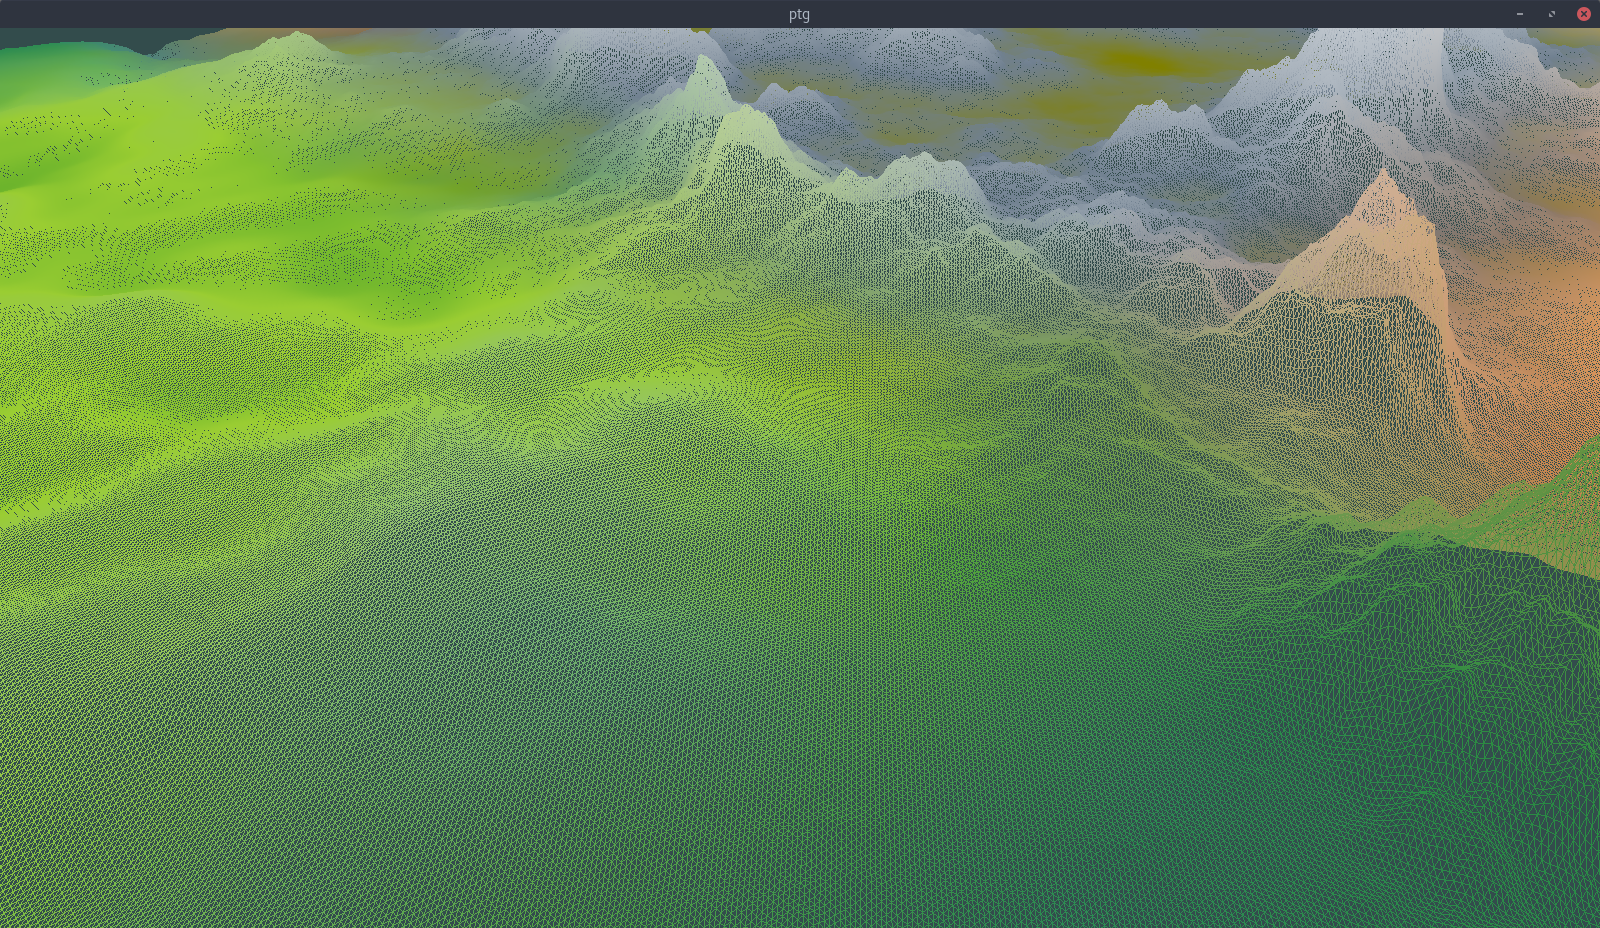
\includegraphics[width=0.48\textwidth]{figuras/wc/wcmi.png}\label{fig:wc_wcmi}}
     
     \caption{Fronteira entre quatro biomas.}
     
     \label{fig:wcborder4biomes}
     % usar \hspace{0.1cm}, é gambiarra mas funciona
\end{figure}

\begin{figure}[H]
     \centering
     \subfloat[][Sem interpolação]{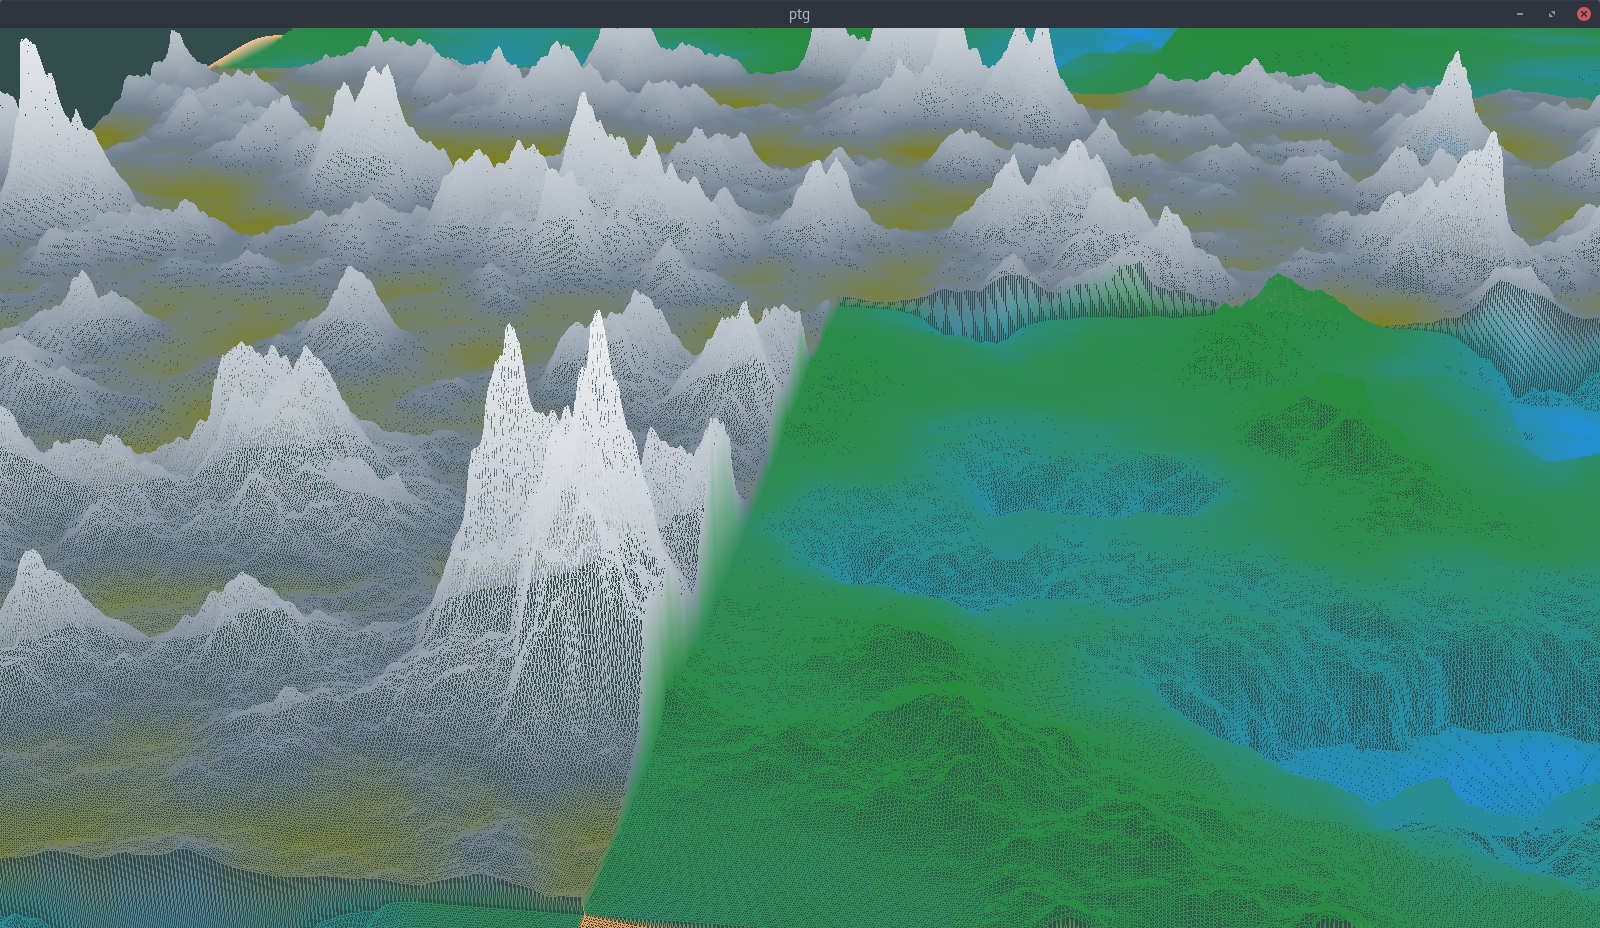
\includegraphics[width=0.48\textwidth]{figuras/borders/0lm.png}\label{fig:borders_0lm}}\hspace{0.1cm}
     \subfloat[][$l = 8$]{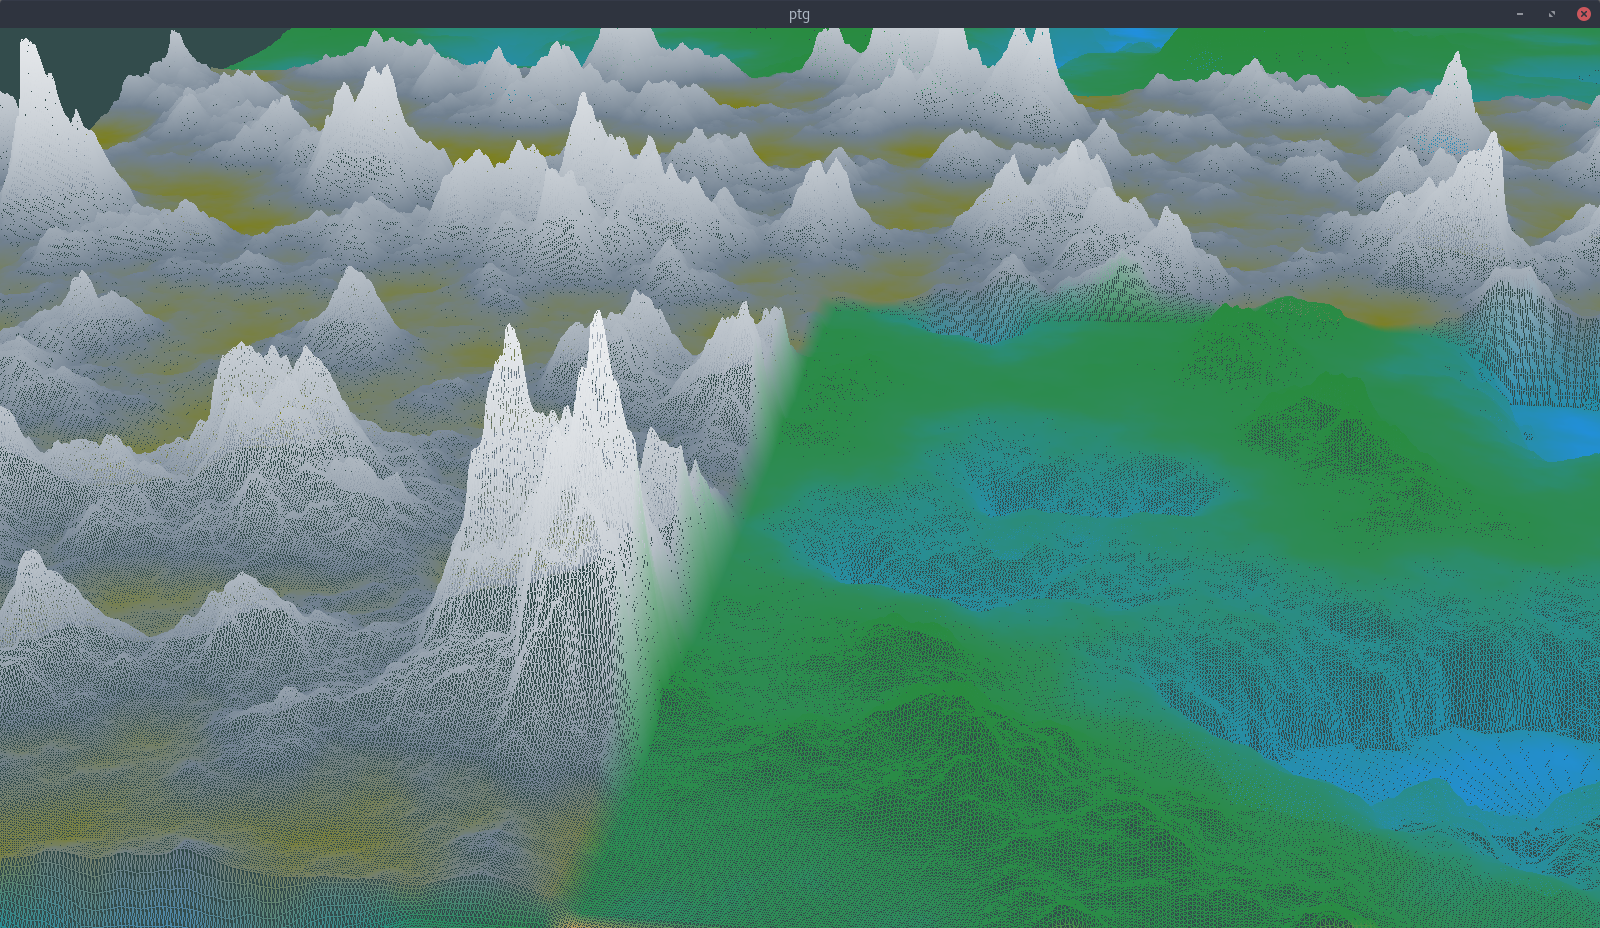
\includegraphics[width=0.48\textwidth]{figuras/borders/8lm.png}\label{fig:borders_8lm}}\\
     \subfloat[][$l = 128$]{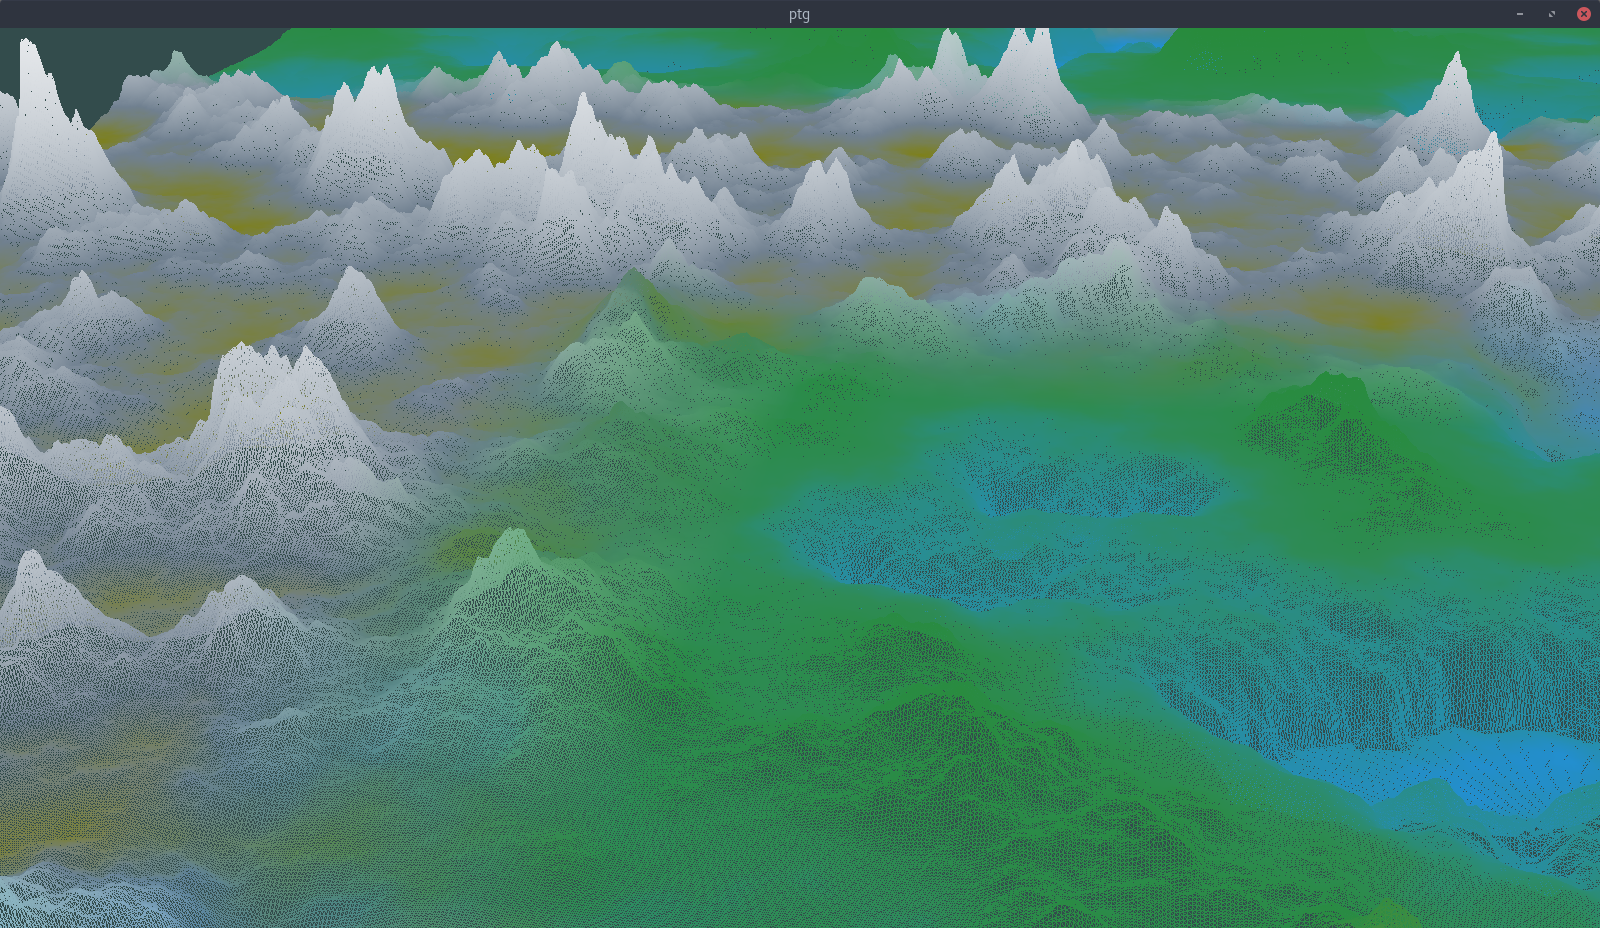
\includegraphics[width=0.48\textwidth]{figuras/borders/128lm.png}\label{fig:borders_128lm}}\hspace{0.1cm}
     \subfloat[][$l = 255$]{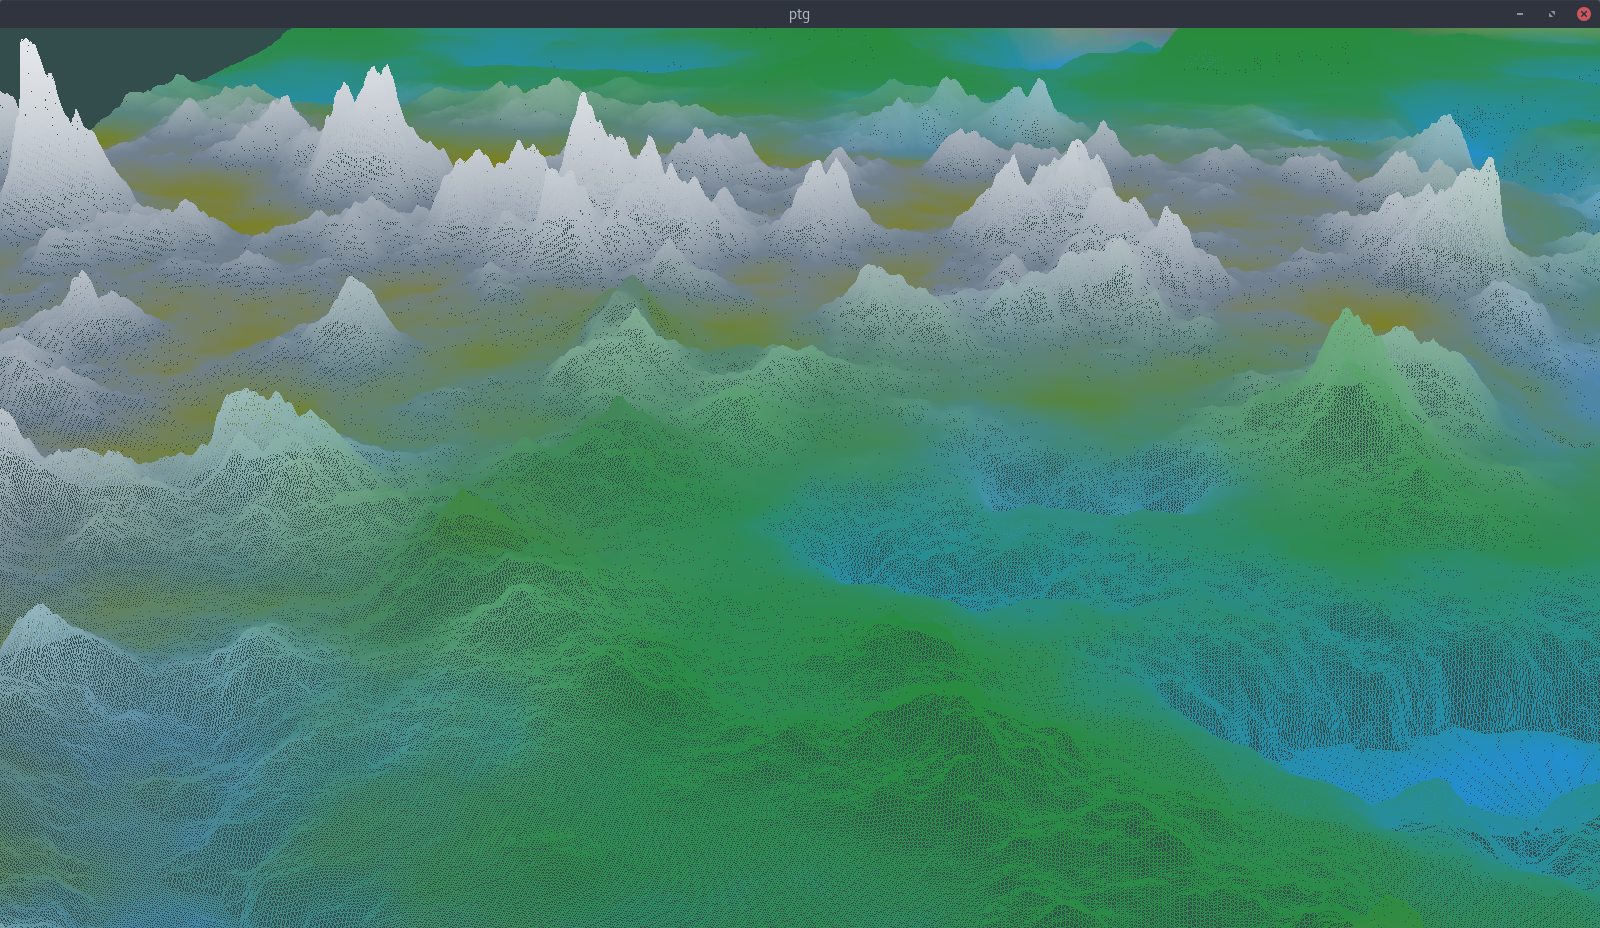
\includegraphics[width=0.48\textwidth]{figuras/borders/255lm.png}\label{fig:borders_255lm}}
     
     
     \caption{Comparando $l$ nas fronteiras.}
     
     \label{fig:borderslcomp}
     % usar \hspace{0.1cm}, é gambiarra mas funciona
\end{figure}






%\begin{figure}[H]
%    \centering
%    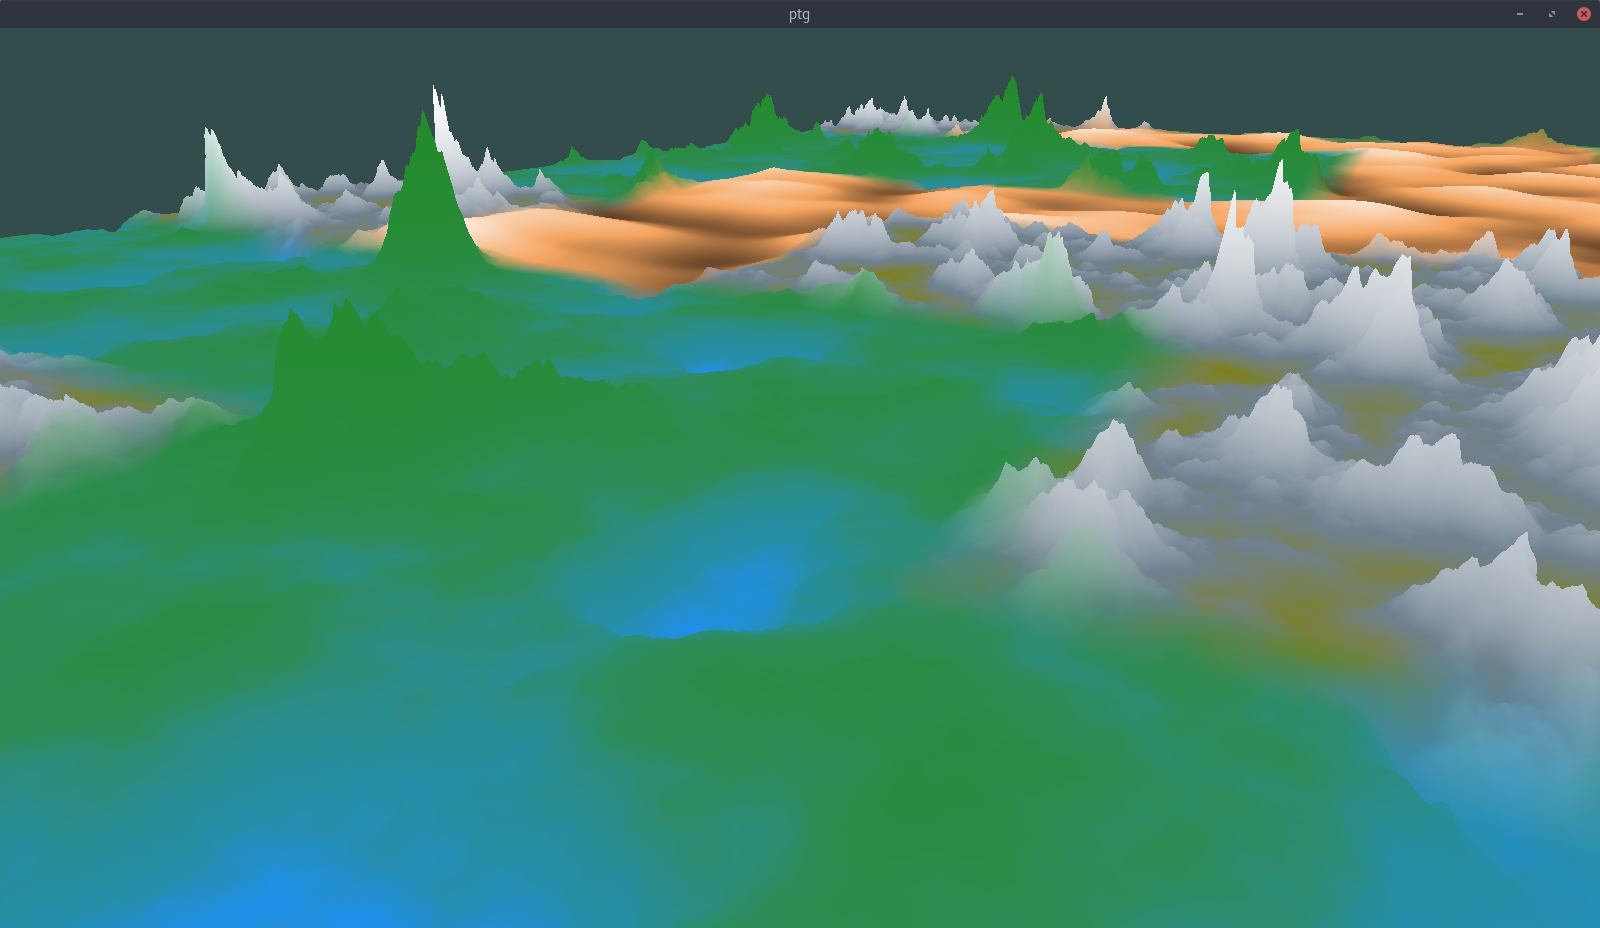
\includegraphics[width=0.5\textwidth]{figuras/ssFinalResult.png}
%    \caption{Resultado final}
%    \label{fig:ssFinalResult}
%\end{figure}
%
%\begin{figure}[H]
%     \centering
%     \subfloat[][$b = 260$]{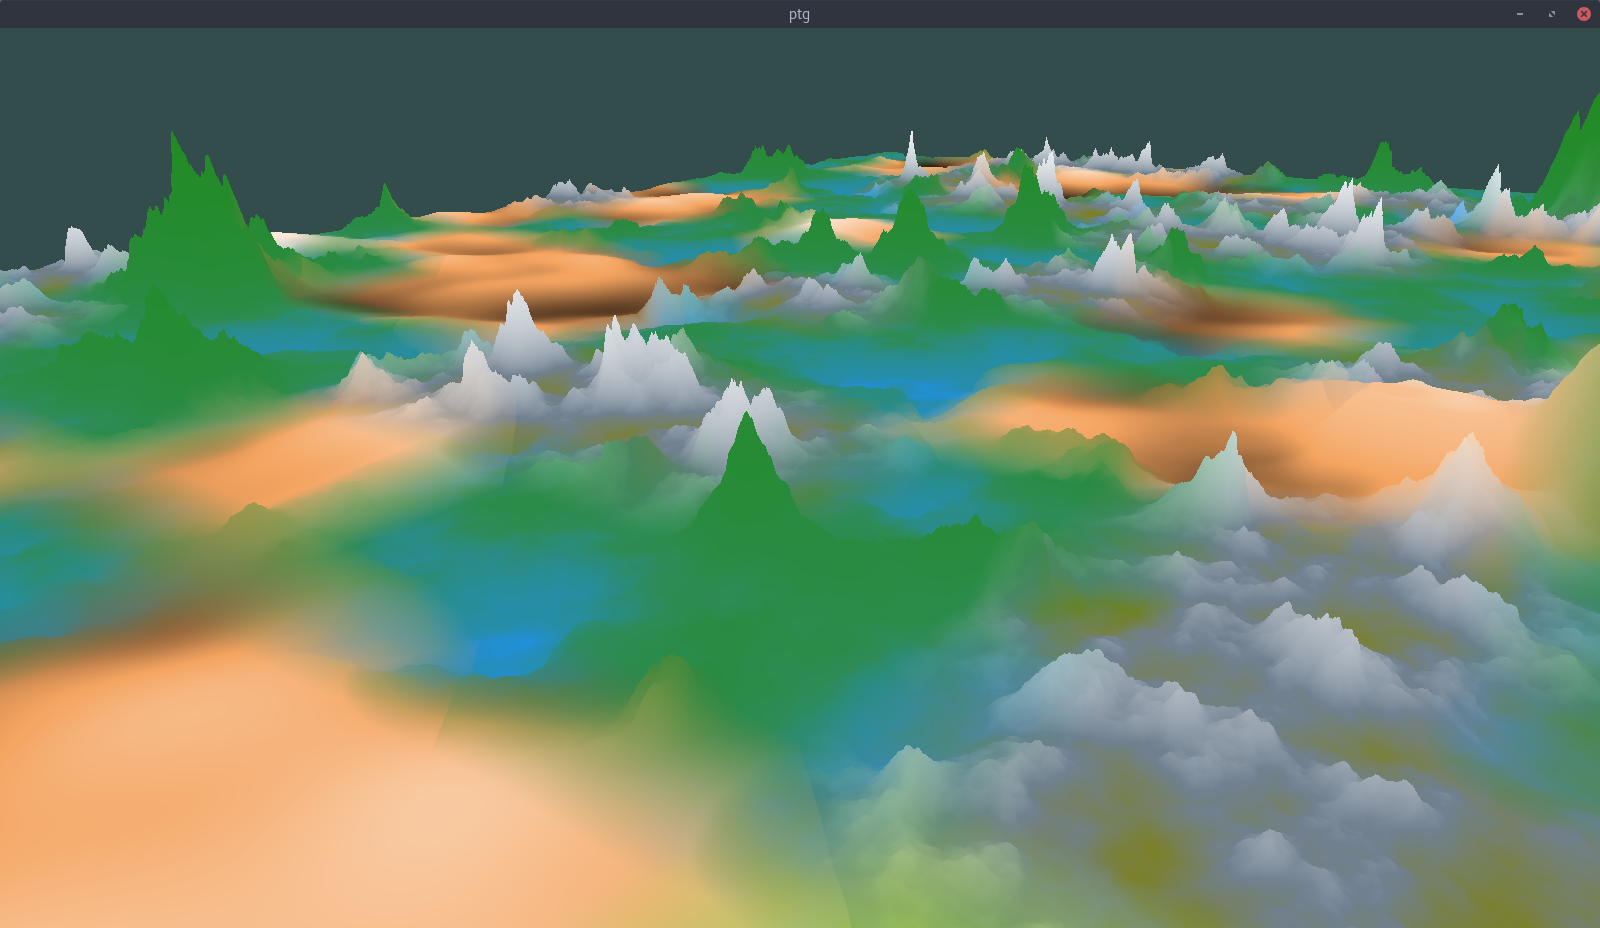
\includegraphics[width=0.48\textwidth]{figuras/resultados/b/resultSeed3Deltav05k2048b260l128.png}\label{fig:b260}}\hspace{0.1cm}
%     \subfloat[][$b = 512$]{\includegraphics[width=0.48\textwidth]{figuras/resultados/b/resultSeed3Deltav05k2048b512l128.png}\label{fig:b512}}\\
%     \subfloat[][$b = 1024$]{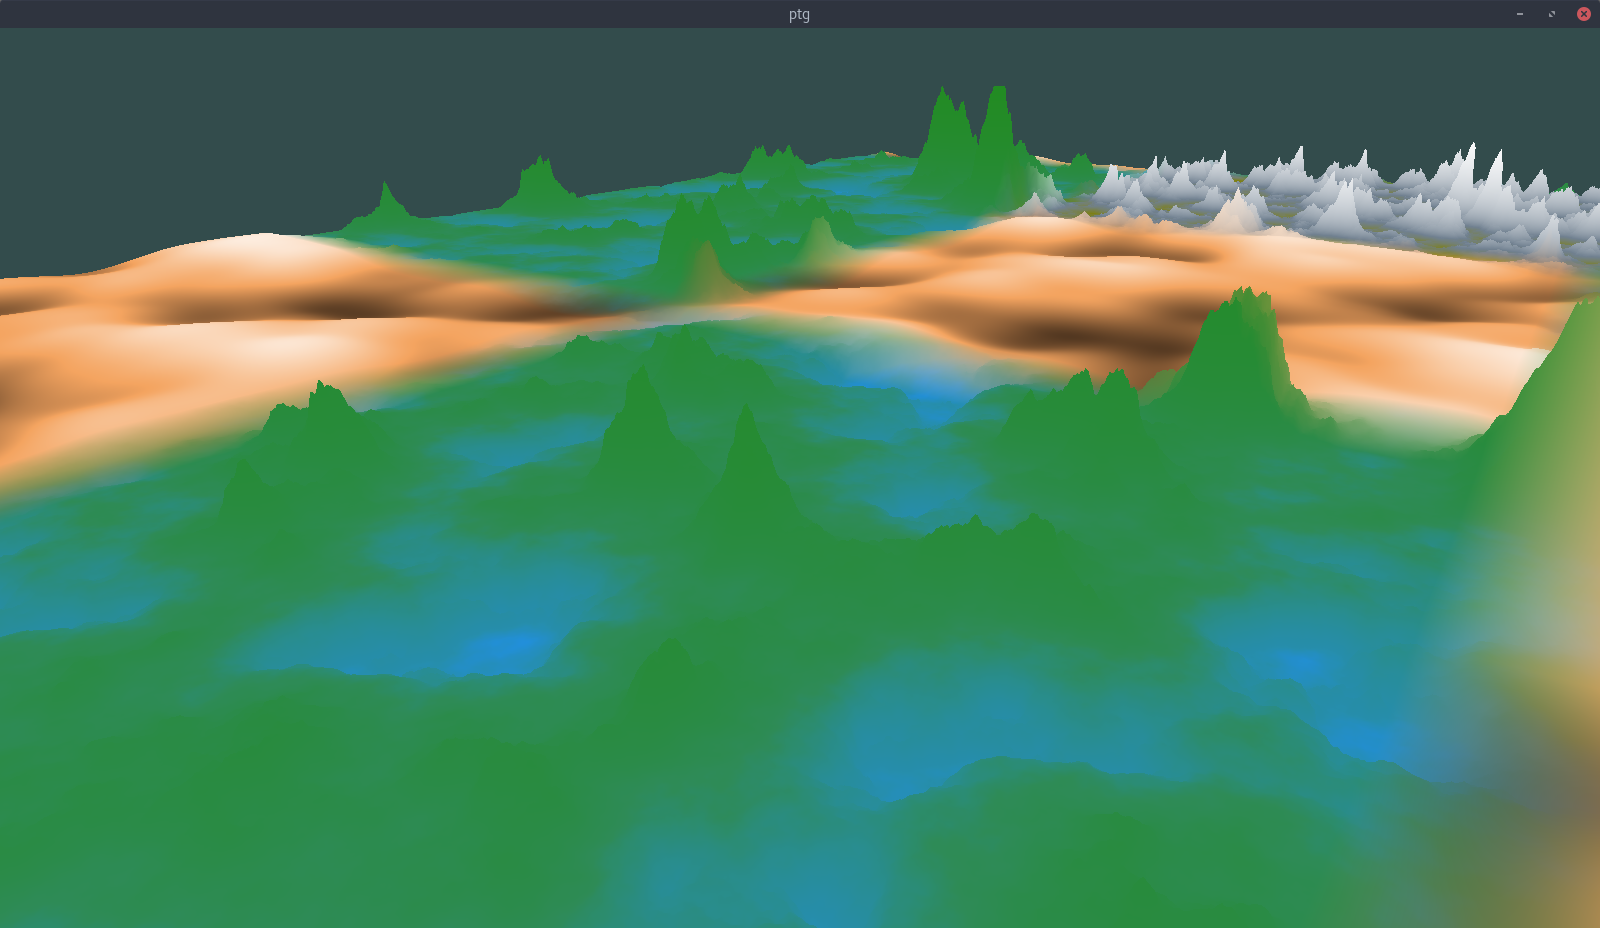
\includegraphics[width=0.48\textwidth]{figuras/resultados/b/resultSeed3Deltav05k2048b1024l128.png}\label{fig:b1024}}\hspace{0.1cm}
%     \subfloat[][$b = 1500$]{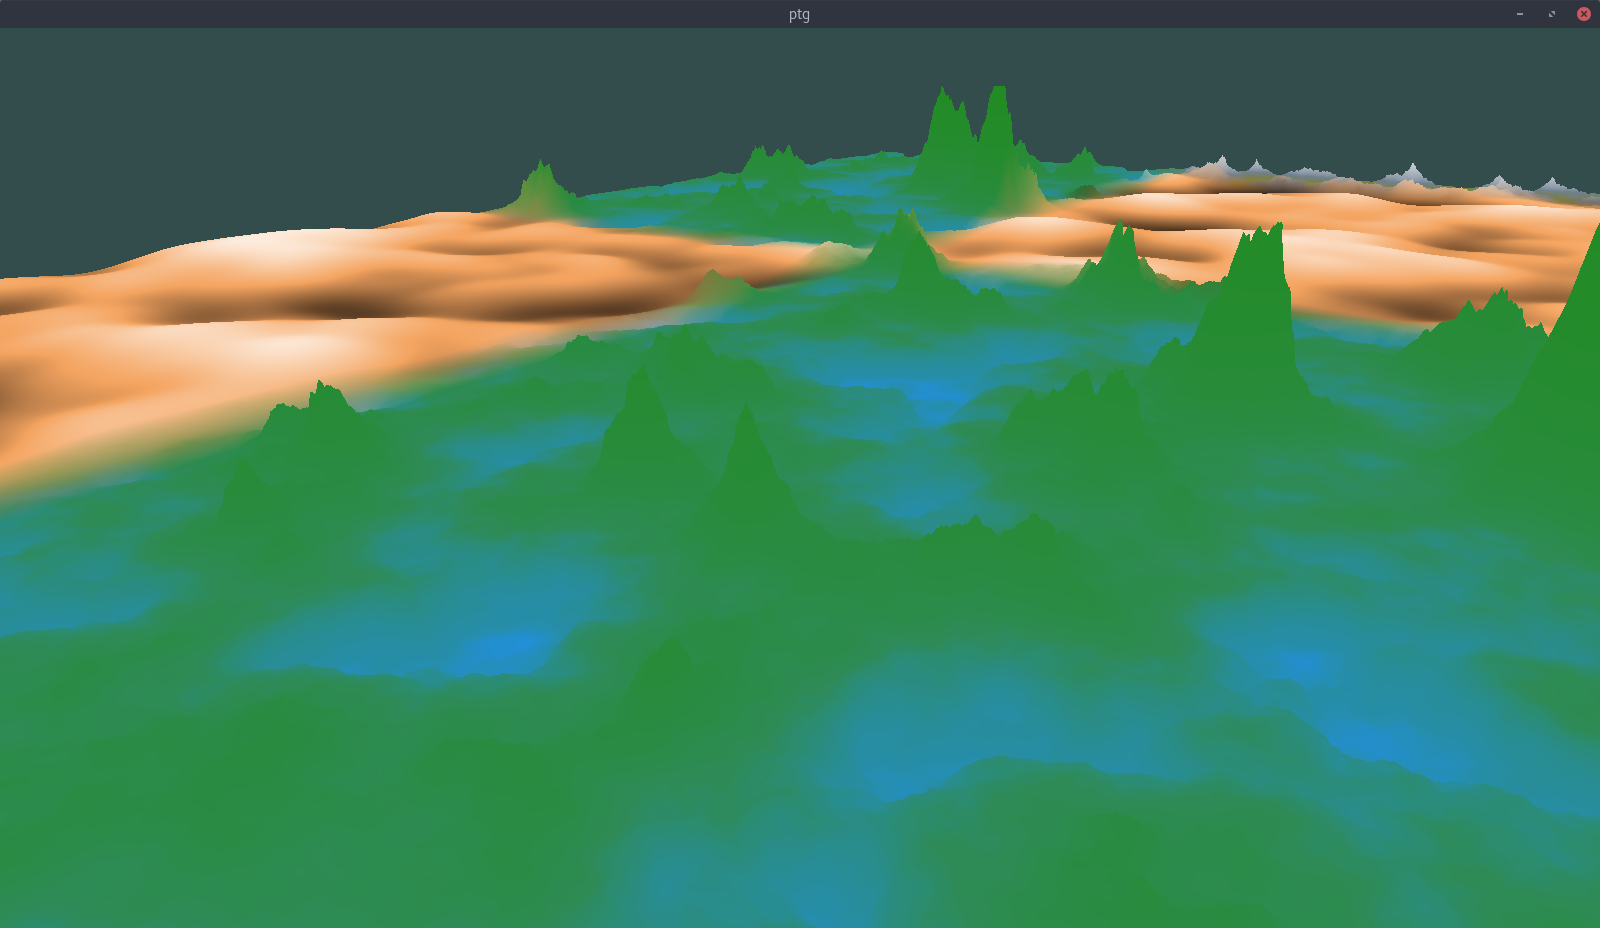
\includegraphics[width=0.48\textwidth]{figuras/resultados/b/resultSeed3Deltav05k2048b1500l128.png}\label{fig:b1500}}
%     
%     \caption{Tamanho de cada Bioma.}
%     
%     \label{fig:biomeComp}
%     % usar \hspace{0.1cm}, é gambiarra mas funciona
%\end{figure}
%
%\begin{figure}[H]
%     \centering
%     \subfloat[][$l = 2$]{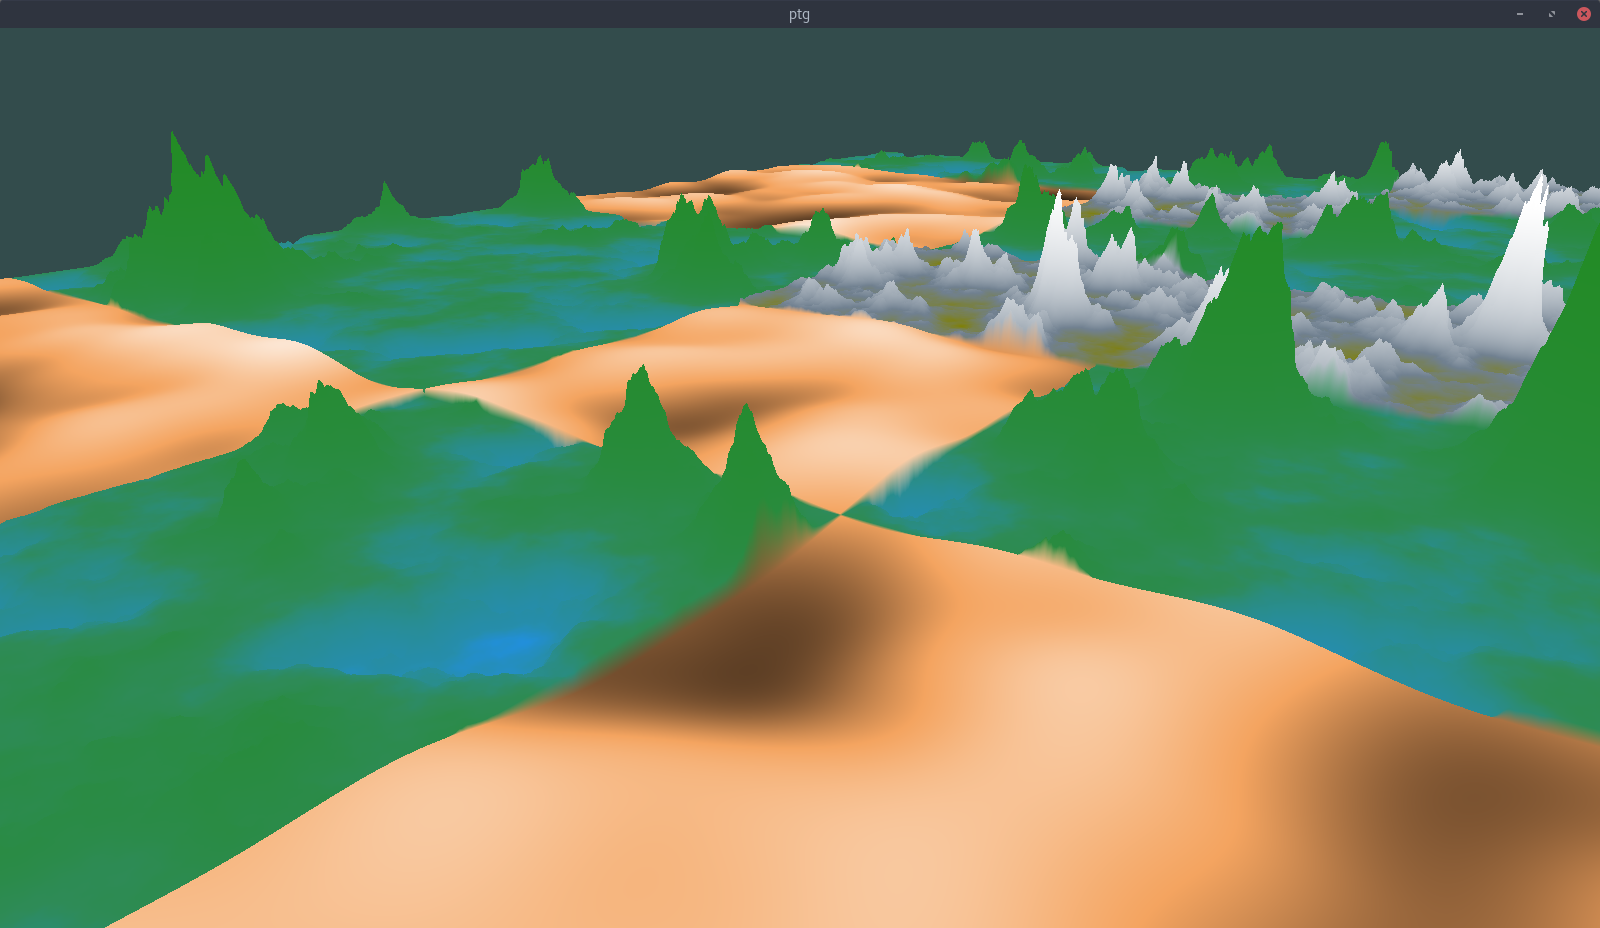
\includegraphics[width=0.48\textwidth]{figuras/resultados/l/resultSeed3Deltav05k2048b512l2.png}\label{fig:l2}}\hspace{0.1cm}
%     \subfloat[][$l = 64$]{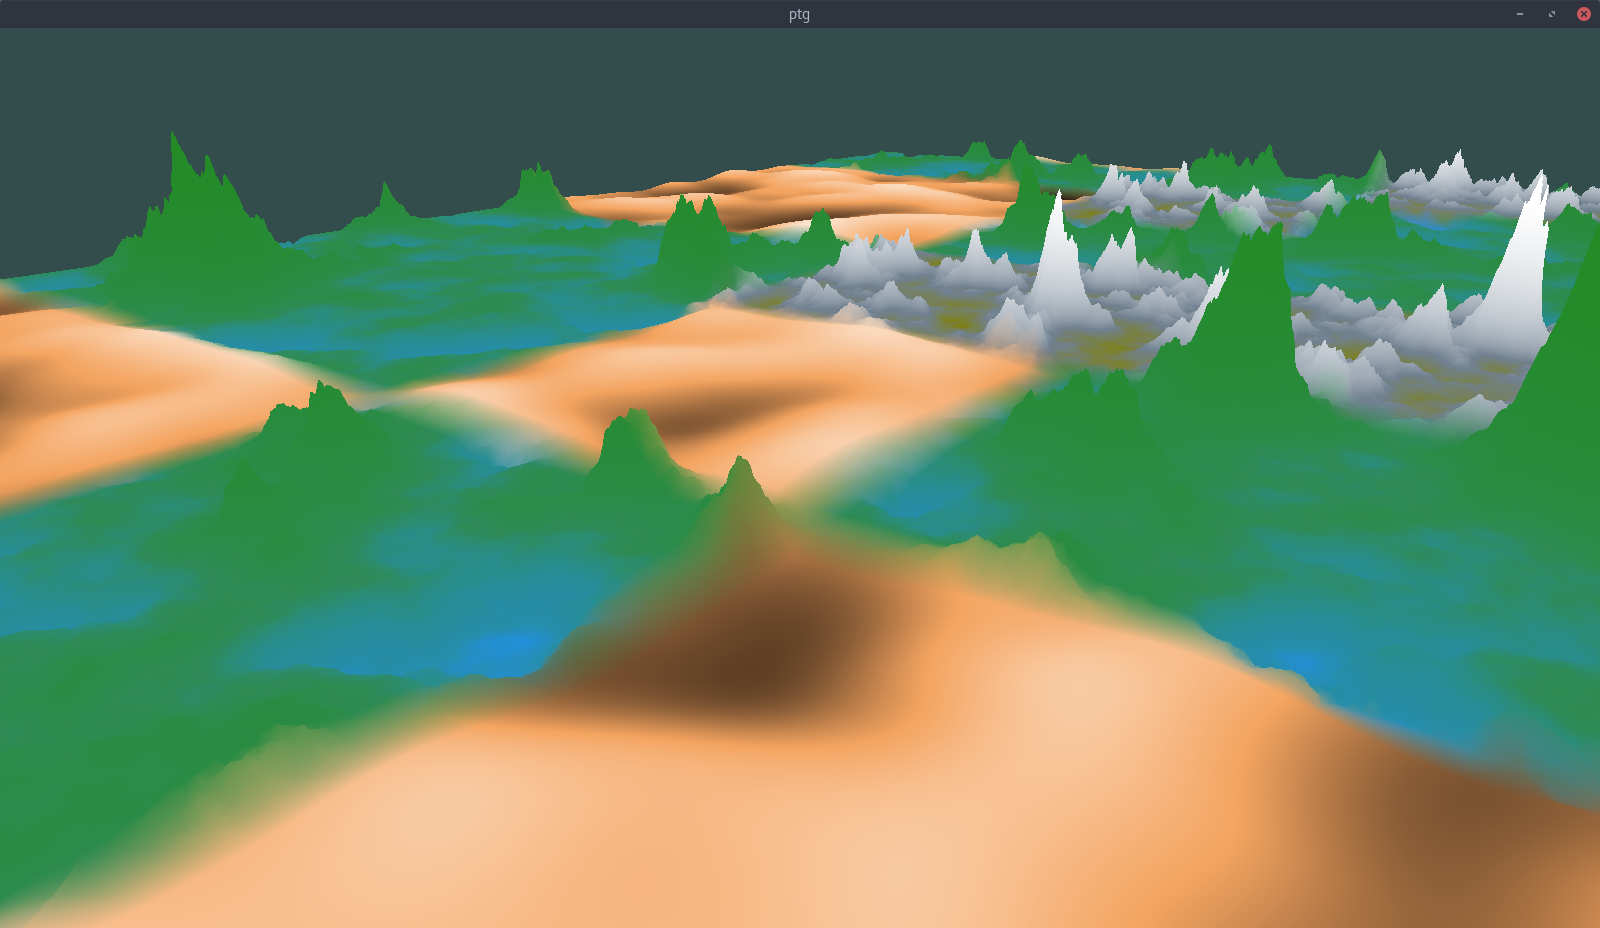
\includegraphics[width=0.48\textwidth]{figuras/resultados/l/resultSeed3Deltav05k2048b512l64.png}\label{fig:l64}}\\
%     \subfloat[][$l = 128$]{\includegraphics[width=0.48\textwidth]{figuras/resultados/l/resultSeed3Deltav05k2048b512l128.png}\label{fig:l128}}\hspace{0.1cm}
%     \subfloat[][$l = 256$]{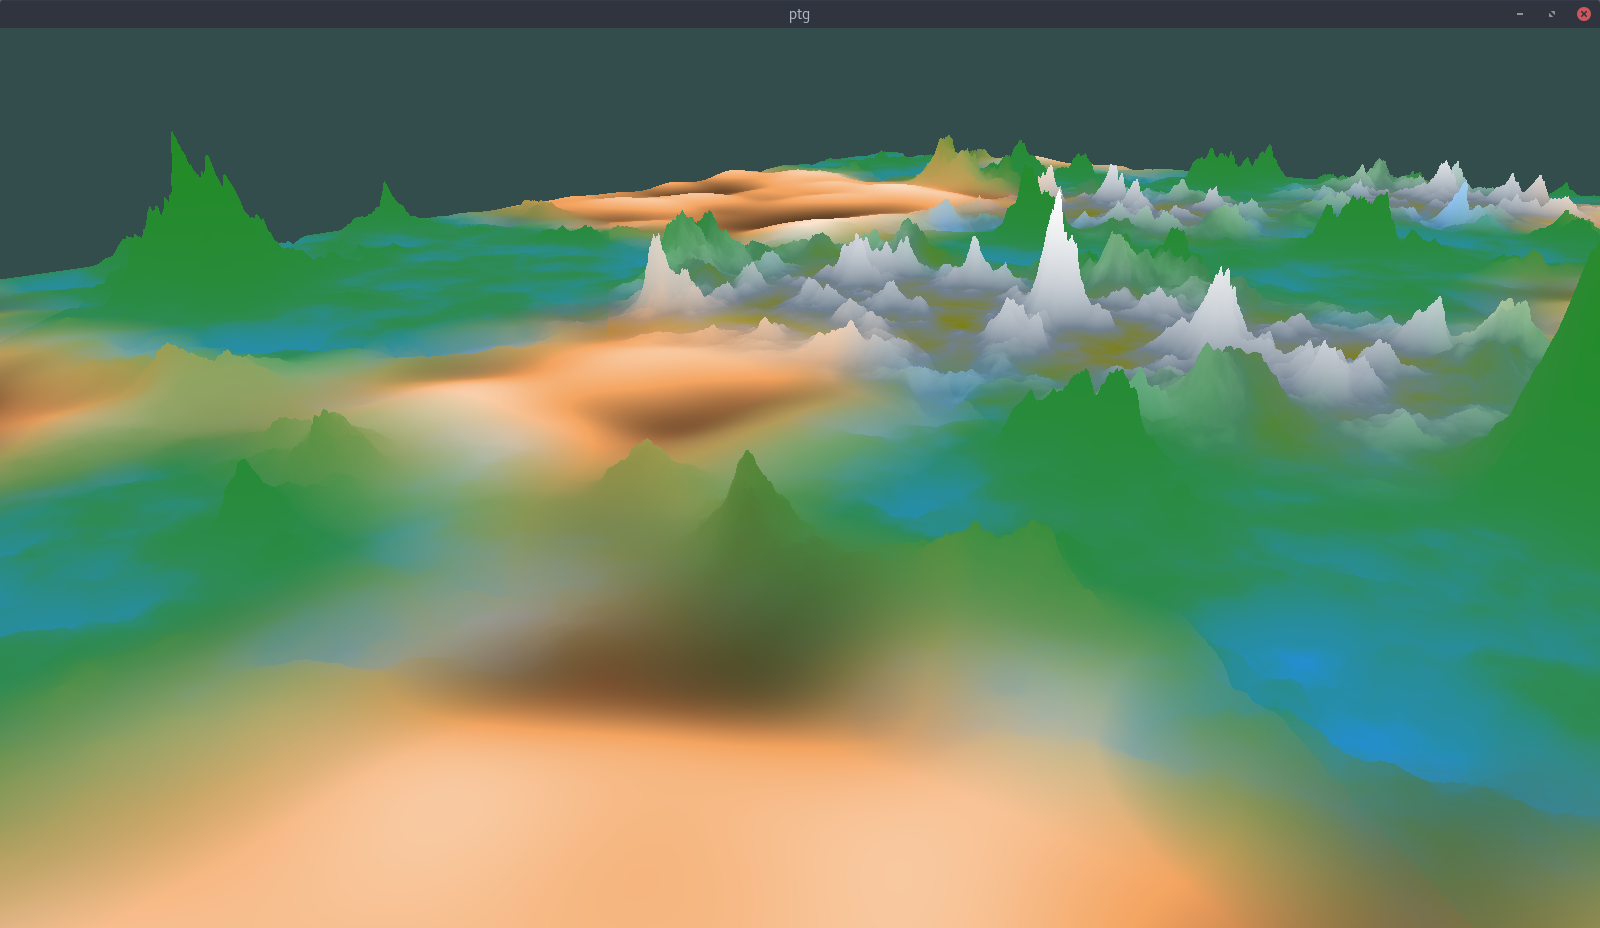
\includegraphics[width=0.48\textwidth]{figuras/resultados/l/resultSeed3Deltav05k2048b512l256.png}\label{fig:l256}}
%     
%     \caption{Alcance da fronteira.}
%     
%     \label{fig:lenghBioComp}
%     % usar \hspace{0.1cm}, é gambiarra mas funciona
%\end{figure}
%
%\begin{figure}[H]
%     \centering
%     \subfloat[][$seed = 1$]{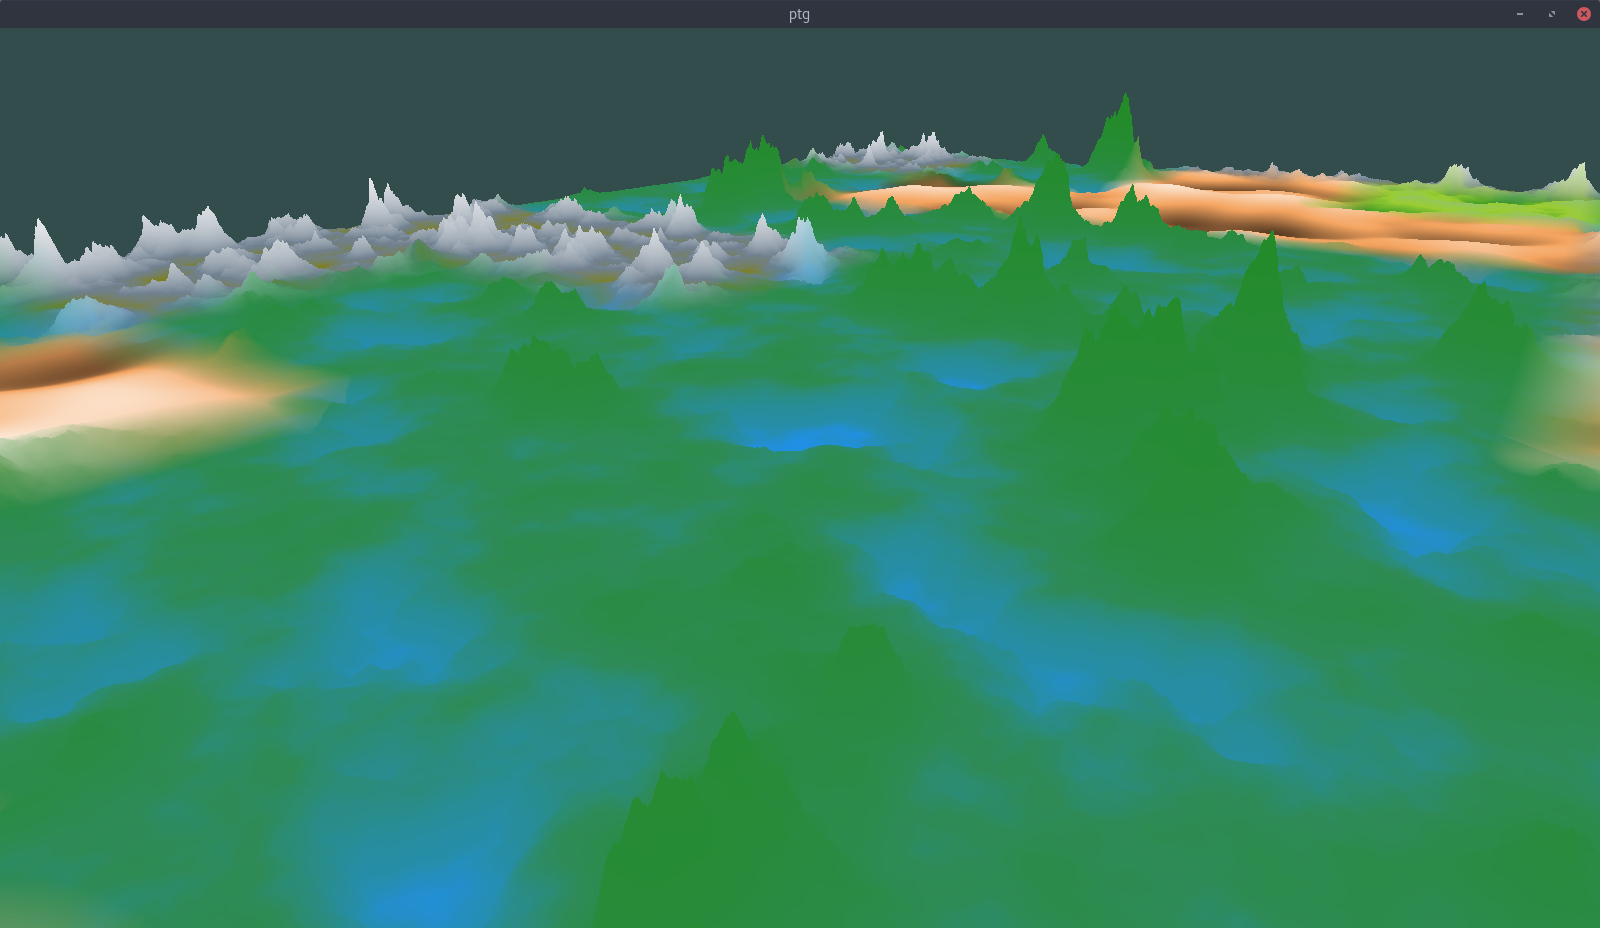
\includegraphics[width=0.48\textwidth]{figuras/resultados/seed/resultSeed1Deltav05k2048b512l128.png}\label{fig:bigseed1}}\hspace{0.1cm}
%     \subfloat[][$seed = 2$]{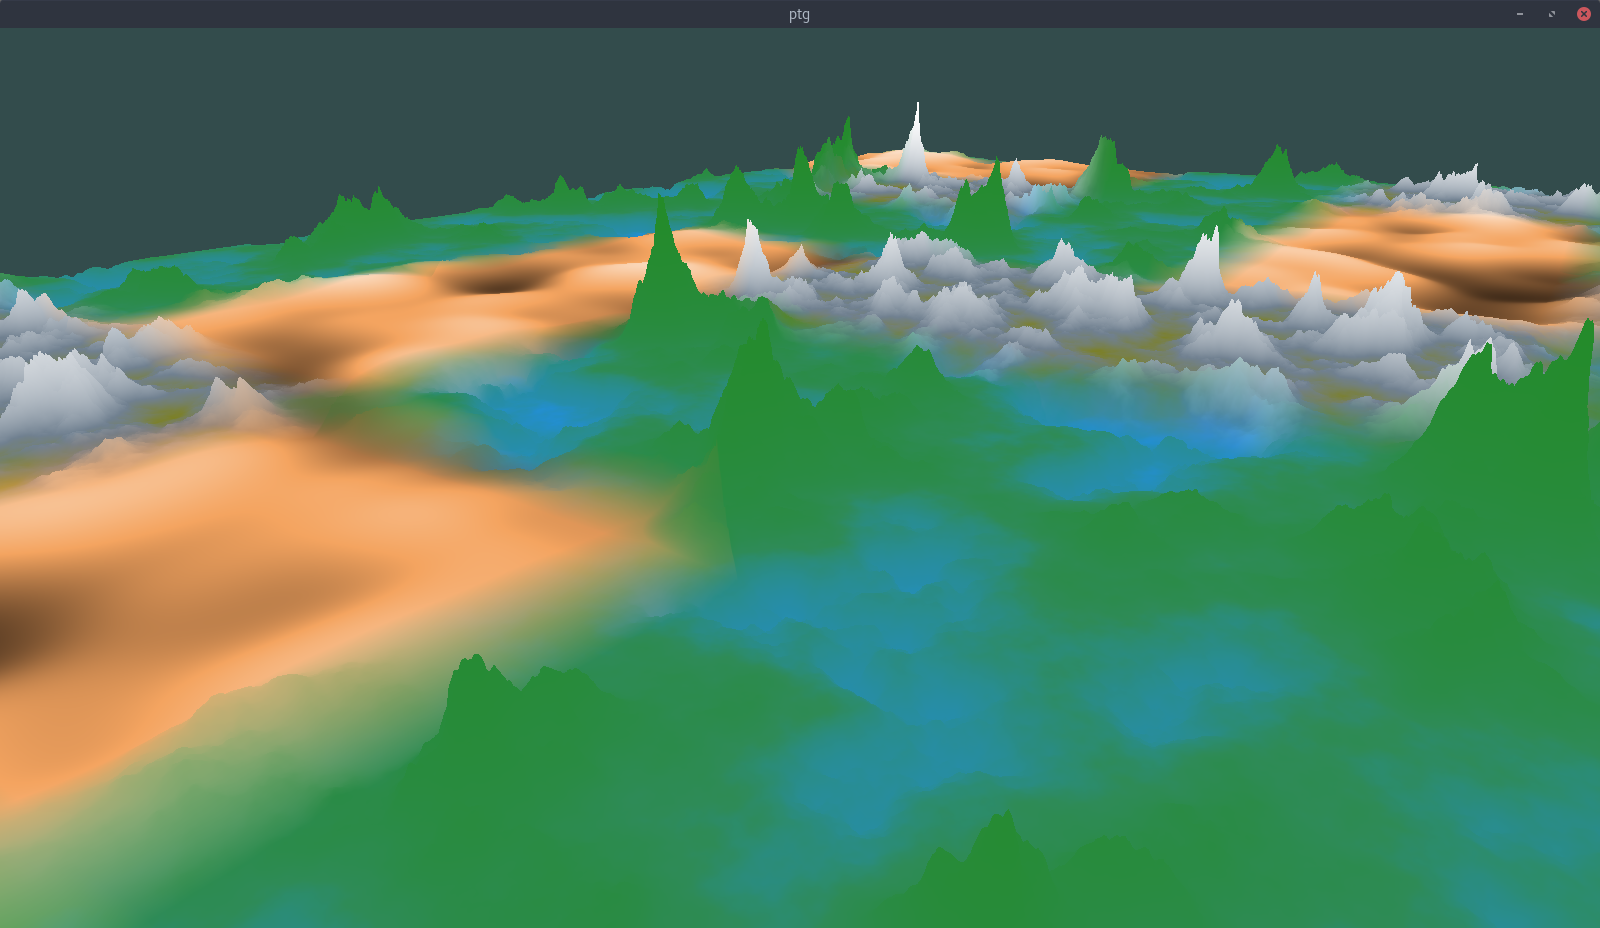
\includegraphics[width=0.48\textwidth]{figuras/resultados/seed/resultSeed2Deltav05k2048b512l128.png}\label{fig:bigseed2}}
%     
%     \caption{Semente para o motor de números pseudo aleatórios.}
%     
%     \label{fig:seedComp}
%     % usar \hspace{0.1cm}, é gambiarra mas funciona
%\end{figure}

%\begin{figure}[H]
%     \centering
%     \subfloat[][$fb = 2$]{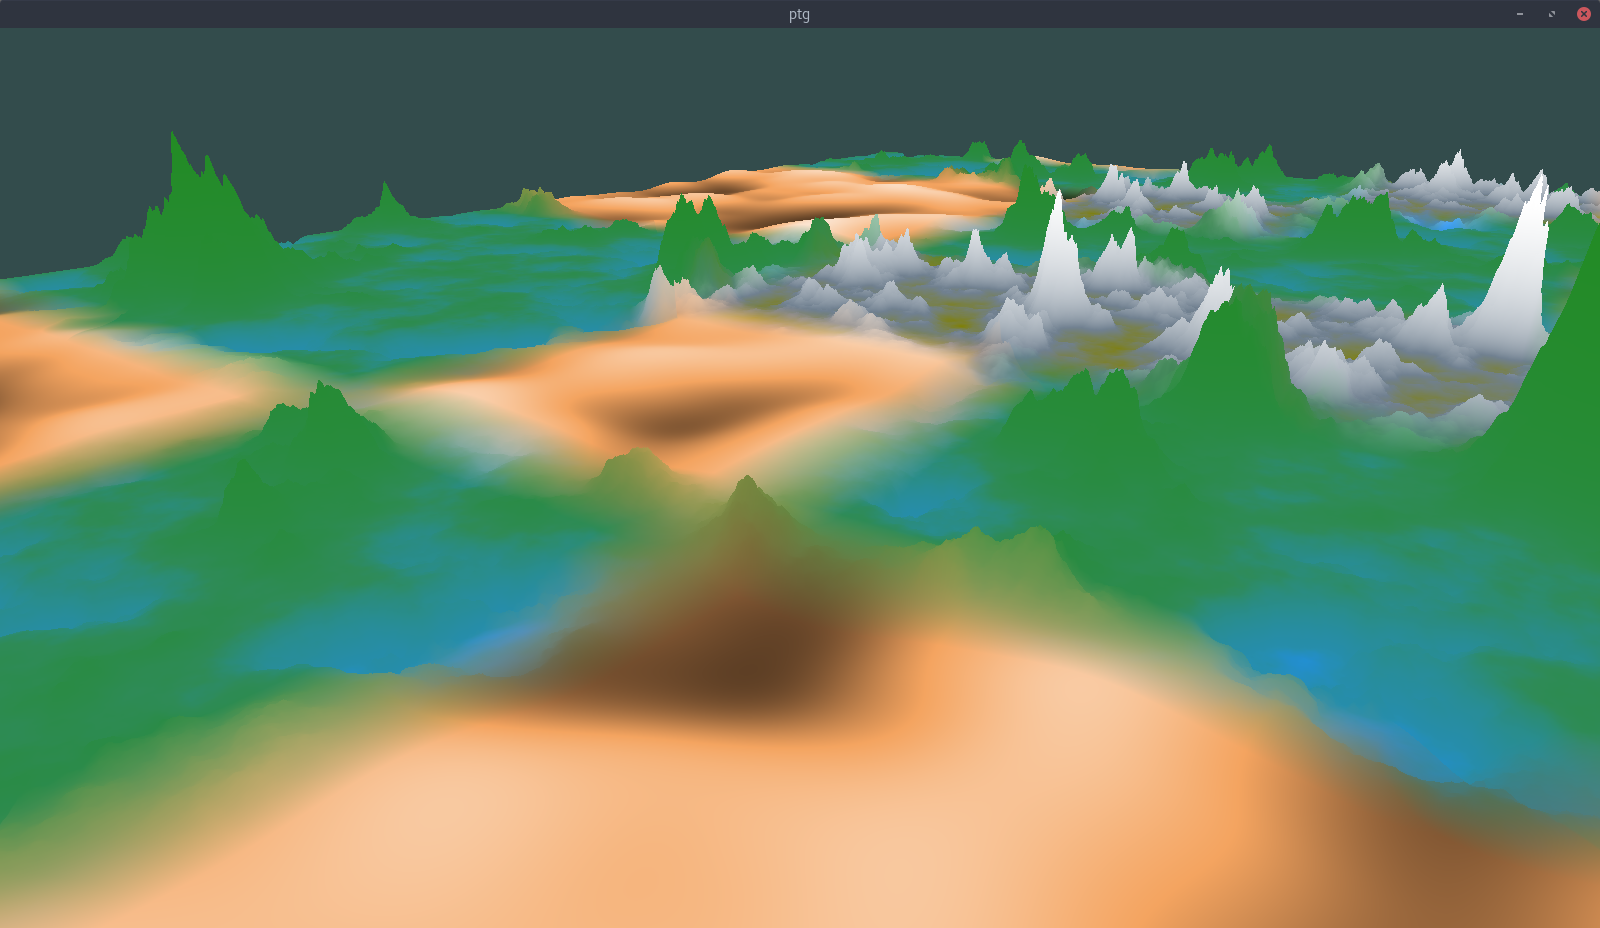
\includegraphics[width=0.48\textwidth]{figuras/resultados/freqb/resultSeed3Deltav05k2048b512l128freqb2.png}\label{fig:freqb2}}\hspace{0.1cm}
%     \subfloat[][$fb = 1/50$]{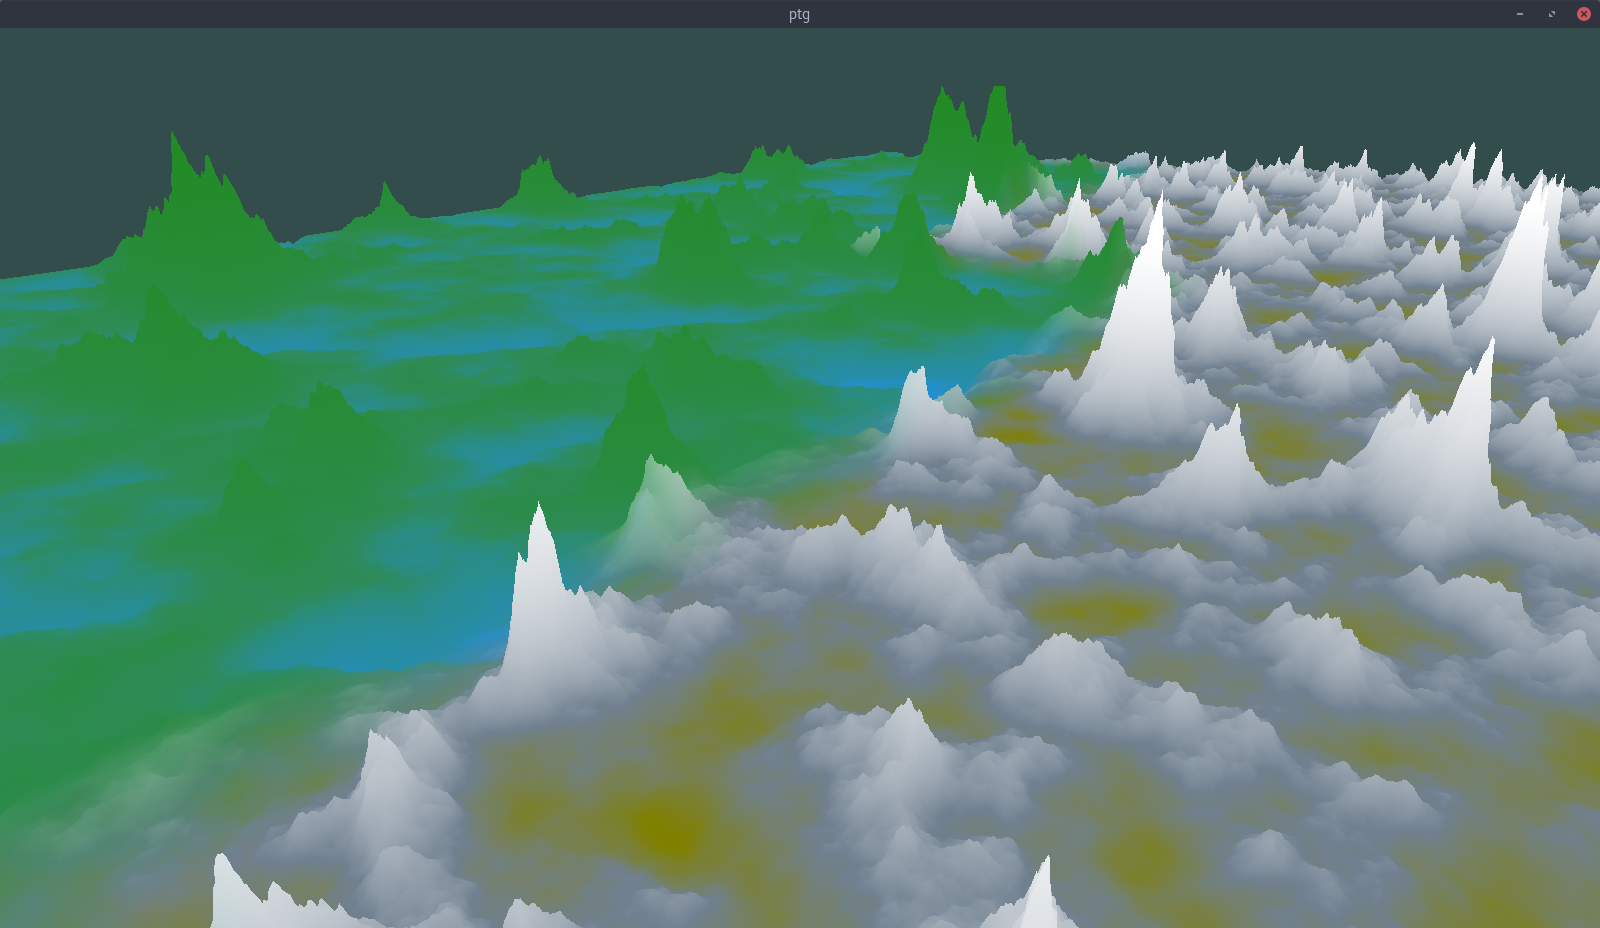
\includegraphics[width=0.48\textwidth]{figuras/resultados/freqb/resultSeed3Deltav05k2048b512l128freqb1_50.png}\label{fig:freqb1_50}}
%     
%     \caption{Frequência de biomas distintos.}
%     
%     \label{fig:freqbComp}
%     % usar \hspace{0.1cm}, é gambiarra mas funciona
%\end{figure}